\begin{SCn}
\scnsectionheader{Предметная область и онтология программных вариантов реализации базового интерпретатора sc-моделей ostis-систем на современных компьютерах}
\begin{scnsubstruct}
    \begin{scnrelfromlist}{соавтор}
    	\scnitem{Зотов Н.В.}
    	\scnitem{Шункевич Д.В.}
   	\end{scnrelfromlist}
    \scnheader{Предметная область программных вариантов реализации базового интерпретатора  sc-моделей ostis-систем на современных компьютерах}
    \scniselement{предметная область}
    \begin{scnhaselementrolelist}{класс объектов исследования}
        \scnitem{ostis-платформа}
    \end{scnhaselementrolelist}
    \begin{scnhaselementrolelist}{ключевой объект исследования}
        \scnitem{Программная платформа ostis-систем}
    \end{scnhaselementrolelist}

    \scnsegmentheader{Спецификация Программной платформы ostis-систем}
	\begin{scnsubstruct}
	\scntext{часто используемый sc-идентификатор}{Документация Программной платформы ostis-систем}
	\scntext{часто используемый sc-идентификатор}{Документация Программного варианта реализации ostis-платформы}
	\scnidtf{База знаний Программного варианта реализации ostis-платформы}
	\scnidtf{Семейство sc-языков, описывающих реализацию компонентов, входящих в состав Программного варианта реализации ostis-платформы (в том числе их программных интерфейсов)}
	\scnidtf{Подробная документация всех компонентов базового Программного варианта реализации ostis-платформы}
	\scnidtf{\textbf{Это пример того, как надо описывать современные программные компьютерные системы}}
	\scniselement{спецификация компонента}
	\scnsubset{База знаний Метасистемы OSTIS}
	\scnrelfrom{автор}{Зотов Н.В.}
	\scntext{идея}{
		Спецификация (документация) такого сложного программного объекта, как \textit{Программная платформа ostis-систем}, может и должна быть представлена на \uline{формальном} \textit{языке представления знаний}, в данном случае на \textit{SC-коде}, тексты которого она хранит и интерпретирует. В таком случае такой язык, который описывает \textit{Программный вариант реализации ostis-платформы}, должен являться \textit{подъязыком} \textit{SC-кода}, то есть должен наследовать все свойства \textit{Синтаксиса} и \textit{Денотационной семантики SC-кода}. Такой способ представления спецификации \textit{программных компьютерных систем} даёт \uline{безусловно} сильные преимущества по сравнению с другими возможными вариантами представления спецификаций \cite{Dillon2008}:
		\begin{itemize}
			\item Язык, тексты которого система хранит и обрабатывает, и язык спецификации того, как система представляет тексты первого языка в памяти самой себя, являются подмножествами \uline{одного и того же} языка. Это упрощает не только становление понимания разработчика, который разрабатывает сложную \textit{программную компьютерную систему}, за счет того, что форма представления обрабатываемого этой системой языка и языка ее спецификации, \uline{унифицирована}, но и позволяет открыть для этой системы новые функциональные возможности в \uline{познании} самой себя. Таким образом, такой подход позволяет полностью реализовывать свойства \textit{интеллектуальной компьютерной системы}, например, \textit{рефлексивности}.
			\item Нельзя проектировать и реализовывать \textit{интеллектуальные компьютерные системы} на \textit{программной компьютерной системе}, которая сама таковой не является. Представление спецификации системы в такой форме позволяет \uline{существенно} повысить уровень ее \textit{интеллекта} \cite{Zagorskiy2022b}.
			\item Нет необходимости в создании дополнительных средств для верификации и анализа работы всей системы, поскольку форма представления языка описания системы \uline{унифицирована} с языком, тексты которого она хранит и интерпретирует. Это позволяет не только уменьшить количество используемых средств при проектировании и реализации такой программной системы, но и позволяет \uline{унифицировать} информацию, хранимую в этой программной системе и описывающую эту программную систему, с целью использования этой информации в процессе эволюции её компонентов. При этом спецификация программной системы остаётся \textit{платформенно-независимой}, поэтому при смене одного варианта реализации \textit{ostis-платформы} на другой подход к описанию таких платформ остаётся \uline{одним и тем же}.
		\end{itemize}
	}
	\scnhaselementrole{ключевой sc-элемент}{\textbf{Программная платформа ostis-систем}}
	\begin{scnindent}
		\begin{scnrelfromset}{общие принципы документирования}
			\scnfileitem{Вне зависимости от языка реализации каждого компонента \textit{Программного варианта реализации ostis-платформы}, спецификация каждого компонента включает спецификацию, непосредственно описанную в \uline{исходных файлах} самого компонента, описывающую программный интерфейс этого компонента, а также спецификацию как \uline{части} базы знаний ostis-платформы, детально описывающую реализацию этого компонента, в том числе используемые алгоритмы.}
			\scnfileitem{\uline{Каждый} компонент \textit{Программного варианта реализации ostis-платформы} описывается средствами \textit{Технологии OSTIS}, то есть на \textit{SC-коде}, тексты которого она обрабатывает и хранит. Таким образом, это дает возможности платформе анализировать свое состояние и способствовать поддерживать свой жизненный цикл без участия ее разработчиков. \textbf{\textit{Программный вариант реализации ostis-платформы} выступает полноценным \uline{субъектом}}, принимающим непосредственное участие в собственной разработке.}
			\scnfileitem{\textit{Спецификация Программного варианта реализации ostis-платформы} представляет собой \uline{\textit{sc-язык}}, то есть подъязык \textit{SC-кода}, для которого уточнены \textit{Cинтаксис} и \textit{Денотационная семантика SC-кода}. Этот \textit{sc-язык} можно представить в виде некоторого семейства более частных sc-языков. Такой подход позволяет без особых препятствий интегрировать описания различных компонентов, входящих в состав \textit{Программного варианта реализации ostis-платформы}, поскольку вся \textit{Спецификация Программного варианта реализации ostis-платформы} является ее базой знаний.}
			\scnfileitem{\uline{Каждый} разработчик \textit{Программного варианта реализации ostis-} \textit{платформы} \uline{заботится} о перманентной поддержки не только состояния ее компонентов, но и спецификации этих компонентов. \uline{Гарантом} качественной \textit{Спецификации Программного варианта реализации ostis-платформы} является ее \uline{коллектив разработчиков}, способных не только понимать детали реализации \textit{ostis-платформы}, но (!) и способствовать к созданию взаимовыгодного сотрудничества для достижения поставленных целей.}
		\end{scnrelfromset}
		\begin{scnindent}
			\scnnote{Данные принципы можно использовать при описании любых (!) других \textit{программных компьютерных систем}, в том числе тех \textit{программных компьютерных систем}, которые не реализуются на данной \textit{ostis-платформе}.}
		\end{scnindent}
		\begin{scnrelfromset}{аналоги}
			\scnitem{Платформа CYC}
			\scnitem{Платформа SMILA}
			\scnitem{Графовая СУБД Neo4j}
			\scnitem{Графовая СУБД OrientDB}
			\scnitem{Графовая СУБД ArangoDB}
			\scnitem{Графовая СУБД Amazon Neptune}
		\end{scnrelfromset}
	\end{scnindent}
	
		
    \scnheader{Программная платформа ostis-систем}
    \scntext{часто используемый sc-идентификатор}{Программный вариант реализации ostis-платформы}
    \scnidtf{Программный вариант реализации базового интерпретатора sc-моделей ostis-систем на традиционных компьютерах}
    \scnidtf{Базовая программная платформа для массового создания интеллектуальных компьютерных систем нового поколения}
    \scnidtf{Программная реализация платформы интерпретации sc-моделей компьютерных систем}
    \scnidtf{Предлагаемый нами программный вариант реализации ассоциативного семантического компьютера}
    \begin{scnindent}
	    \scntext{пояснение}{Одним из путей, позволяющих осуществлять апробацию, развитие, а в ряде случаев и внедрение новых моделей и технологий вне зависимости от наличия соответствующих аппаратных средств является разработка программных моделей этих аппаратных средств, которые были бы функционально эквивалентны этим аппаратным средствам, но при этом интерпретировались на базе традиционной аппаратной архитектуры (в данной работе традиционной архитектурой будем считать архитектуру фон Неймана, как доминирующую в настоящее время). Очевидно, что производительность таких программных моделей в общем случае будет ниже, чем самих аппаратных решений, однако в большинстве случаев она оказывается достаточной для того, чтобы развивать соответствующую технологию параллельно с разработкой аппаратных средств и осуществления постепенного перевода уже работающих систем с программной модели на аппаратные средства.}
    \end{scnindent}
    \scnidtf{Реализация sc-машины}
    \scnidtf{sc-machine}
    \scniselement{базовая ostis-платформа}
    \scniselement{web-ориентированный вариант реализации ostis-платформы}
    \begin{scnindent}
    	\scnidtf{вариант реализации платформы интерпретации sc-моделей компьютерных систем, предполагающий взаимодействие пользователей с системой \uline{посредством} сети Интернет}
    \end{scnindent}
    \scniselement{многопользовательский вариант реализации ostis-платформы}
    \scniselement{многократно используемый компонент ostis-систем, хранящийся в виде файлов исходных текстов}
   	\scniselement{платформенно-зависимый многократно используемый компонент ostis-систем}
	\scniselement{неатомарный многократно используемый компонент ostis-систем}
    \scniselement{зависимый многократно используемый компонент ostis-систем}
    \scntext{адрес компонента}{https://github.com/ostis-ai/sc-machine}
    \begin{scnrelfromset}{декомпозиция программной системы}
    	\scnitem{Реализация sc-памяти}
    	\scnitem{Реализация scp-интерпретатора}
		\begin{scnindent}
			\scnsuperset{Реализация интерпретатора сетевого взаимодействия между ostis-системами}
    		\scnsuperset{Реализация интерпретатора sc-моделей пользовательских интерфейсов ostis-систем}
    	\end{scnindent}
    	\scnitem{Реализация менеджера многократно используемых компонентов ostis-систем}
    \end{scnrelfromset}
    \begin{scnrelfromset}{зависимости компонента}
    	\scnitem{Реализация sc-памяти в ostis-платформе}
    \end{scnrelfromset}
	\scntext{принципы реализации}{Поскольку sc-тексты представляют собой семантические сети, то есть, по сути, графовые конструкции определенного вида, то на нижнем уровне задача разработки программного варианта реализации платформы интерпретации sc-моделей сводится к разработке средств хранения и обработки таких графовых конструкций.К настоящему времени разработано большое количество простейших моделей представления графовых конструкций в линейной памяти, таких как матрицы смежности, списки смежности и другие (\cite{Diskrete_Math}). Однако, при разработке сложных систем как правило приходится использовать более эффективные модели, как с точки зрения объема информации, требуемого для представления, так и с точки зрения эффективности обработки графовых конструкций, хранимых в той или иной форме. К наиболее распространенным программным средствам, ориентированным на хранение и обработку графовых конструкций относятся графовые СУБД (Neo4j \cite{Neo4j}, ArangoDB \cite{ArangoDB}, OrientDB \cite{OrientDB}, Grakn \cite{Grakn} и др.), а также так называемые rdf-хранилища (Virtuoso \cite{Virtuoso}, Sesame \cite{Sesame} и др.), предназначенные для хранения конструкций, представленных в модели RDF. Для доступа к информации, хранимой в рамках таких средств, могут использоваться как языки, реализуемые в рамках конкретного средства (например, язык Cypher в Neo4j), так и языки, являющиеся стандартами для большого числа систем такого класса (например, SPARQL для rdf-хранилищ).Популярность и развитость такого рода средств приводит к тому, что на первый взгляд целесообразным и эффективным кажется вариант реализации \textit{программного варианта реализации платформы интерпретации sc-моделей} на базе одного из таких средств. Однако, существует ряд причин, по которым было принято решение о реализации \textit{программного варианта реализации платформы интерпретации sc-моделей} с нуля. К ним относятся следующие:
	\begin{scnitemize}
		\item Для обеспечения эффективности хранения и обработки \textit{информационных конструкций} определенного вида (в данном случае --- \textit{sc-конструкций}), должна учитываться специфика этих конструкций. В частности, описанные в работе \cite{Koronchik2013a} эксперименты показали значительный прирост эффективности собственного решения по сравнению с существующими на тот момент.   	
		\item В отличие от классических \textit{графовых конструкций}, где \textit{дуга} или \textit{ребро} могут быть инцидентны только \textit{узлу} \textit{графа} (это справедливо и для \textit{rdf-графов}) в \textit{SC-коде} вполне типичной является ситуация, когда \textit{sc-коннектор} инцидентен другому \textit{sc-коннектору} или даже двум \textit{sc-коннекторам} \cite{Ivashenko2022}. В связи с этим существующие средства хранения \textit{графовых конструкций} не позволяют в явном виде хранить \textit{sc-конструкции} (\textit{sc-графы}). Данная проблема также решаема при переходе от \textit{неориентированного графа} к \textit{орграфу} \cite{Ivashenko2015}.
		\item В основе обработки информации в рамках \textit{Технологии OSTIS} лежит \textit{многоагентный подход} \cite{Shunkevich2022a}, в рамках которого агенты обработки информации, хранимой в sc-памяти (sc-агенты) реагируют на события, происходящие в sc-памяти и обмениваются информацией посредством спецификации выполняемых ими действий в sc-памяти \cite{Shunkevich2018}. В связи с этим одной из важнейших задач является реализация в рамках \textit{Программного варианта реализации ostis-платформы} возможности подписки на события, происходящие в программной модели sc-памяти, которая на данный момент практически не поддерживается в рамках современных средств хранения и обработки графовых конструкций.
		\item \textit{SC-код} позволяет описывать также внешние \textit{информационные конструкции} любого рода (изображения, текстовые файла, аудио- и видеофайлы и так далее \cite{Ivashenko2022}, которые формально трактуются как содержимое \textit{sc-элементов}, являющихся знаками \textit{внешних файлов ostis-системы}. Таким образом, компонентом \textit{Программного варианта ostis-платформы} должна быть реализация файловой памяти, которая позволяет хранить указанные конструкции в каких-либо общепринятых форматах. Реализация такого компонента в рамках современных средств хранения и обработки \textit{графовых конструкций} также не всегда представляется возможной.
	\end{scnitemize}
	По совокупности перечисленных причин было принято решение о реализации \textit{программного варианта реализации платформы интерпретации sc-моделей} \scnqq{с нуля} с учетом особенностей хранения и обработки информации в рамках Технологии OSTIS.}
    \begin{scnrelfromset}{особенности реализации}
    	\scnfileitem{Текущий \textit{Программный вариант реализации ostis-платформы} является \uline{web-ориентированным}, поэтому с этой точки зрения каждая \mbox{ostis-система} представляет собой web-сайт, доступный онлайн посредством обычного браузера. Такой вариант реализации обладает очевидным преимуществом --- доступ к системе возможен из любой точки мира, где есть Интернет, при этом для работы с системой не требуется никакого специализированного программного обеспечения. С другой стороны, такой вариант реализации обеспечивает возможность параллельной работы нескольких пользователей с системой.}
    	\scnfileitem{Реализация является \uline{\textit{кроссплатформенной}} и может быть собрана из исходных текстов в различных \textit{операционных системах}. В то же время, взаимодействие клиентской и серверной части организовано таким образом, что \mbox{web-интерфейс} может быть легко заменен на настольный или мобильный интерфейс, как универсальный, так и специализированный.}
    	\scnfileitem{Текущий вариант реализации ostis-платформы является \uline{базовым}, то есть включает \textit{Реализацию scp-интерпретатора}).}
    	\scnfileitem{\uline{Ядром} этой платформы является \textit{Реализация sc-памяти}. Текущая \textit{Реализация sc-памяти} \uline{функционально полна}, то есть позволяет хранить \textit{sc-конструкции}, с помощью которых описывается любая \textit{sc-модель ostis-системы}, внешние \textit{информационные конструкции}, не принадлежащие \textit{SC-коду}, а также предоставлять различные уровни доступа для обработки этих конструкций. В контексте текущего \textit{Программного варианта реализации ostis-платформы} \textit{Реализация sc-памяти} включает \textit{Реализацию файловой памяти}, предназначенной для хранения внешних \textit{информационных конструкций}, не принадлежащих \textit{SC-коду}, то есть содержимое \textit{внутренних файлов ostis-системы}, но дополнительно описывающие, поясняющие и детализирующие \textit{sc-конструкции} \textit{sc-моделей ostis-систем}.}
    	\scnfileitem{Текущий \textit{Программный вариант реализации ostis-платформы} включает \textit{Реализацию менеджера многократно используемых компонентов ostis-систем}. В первую очередь это связано с тем, что текущая \textit{Реализация менеджера многократно используемых компонентов ostis-систем} использует \textit{Реализацию sc-памяти ostis-платформы} для хранения и обработки спецификаций устанавливаемых компонентов вне зависимости от языка их реализации, а также является платформенно-зависимым многократно используемым компонентом ostis-систем.}
    \end{scnrelfromset}
	
	\scnsegmentheader{Спецификация Реализации sc-памяти в Программной платформе ostis-систем}
	\begin{scnsubstruct}
	\scnidtf{Документация Реализации sc-памяти в Программной платформе ostis-систем}
	\scnhaselementrole{ключевой sc-элемент}{\textbf{Реализация sc-памяти}}

	\scnheader{Реализация sc-памяти}
	\scnidtf{Программный вариант реализации графодинамической ассоциативной памяти в Программной платформе ostis-систем}
 	\scnidtf{Программная модель семантической памяти, реализованная на основе традиционной линейной памяти и включающая средства хранения sc-конструкций и базовые средства для обработки доступа к этим конструкциям, в том числе удаленного доступа к ним посредством соответствующих сетевых языков (протоколов)}
	\scnidtf{Предлагаемый нами вариант реализации графодинамической ассоциативной памяти для ostis-систем}
	\scniselement{реализация sc-памяти}
	\scniselement{многократно используемый компонент ostis-систем, хранящийся в виде файлов исходных текстов}
	\scniselement{платформенно-зависимый многократно используемый компонент ostis-систем}
	\scniselement{неатомарный многократно используемый компонент ostis-систем}
	\scniselement{зависимый многократно используемый компонент ostis-систем}
	\scnrelto{программная модель}{sc-память}
	\begin{scnindent}
		\scnrelto{семейство подмножеств}{сегмент sc-памяти}
		\begin{scnindent}
			\scnidtf{страница sc-памяти}
	 		\scntext{пояснение}{В рамках данного \textit{Программного варианта реализации ostis-платформы} \textit{sc-память} моделируется в виде набора \textit{сегментов}, каждый из которых представляет собой фиксированного размера упорядоченную последовательность \textit{элементов sc-памяти}, каждый из которых соответствует конкретному \textit{sc-элементу}.}
			\scnrelto{семейство подмножеств}{элемент sc-памяти}
			\begin{scnindent}
				\scntext{пояснение}{В настоящее время каждый сегмент состоит из $2^{16}-1=65535$ \textit{элементов sc-памяти}. Каждый сегмент состоит из набора структур данных, описывающих конкретные \textit{sc-элементы} (элементов sc-памяти). Независимо от типа описываемого sc-элемента каждый \textit{элемент sc-памяти} имеет фиксированный размер (в текущий момент --- 44 байт), что обеспечивает удобство их хранения. Таким образом, максимальный размер базы знаний в текущей программной модели sc-памяти может достигнуть 223 Гб (без учета содержимого \textit{внутренних файлов ostis-системы}, хранимого в файловой памяти).}
			\end{scnindent}
			\scntext{примечание}{Выделение \textit{сегментов sc-памяти} позволяет, с одной стороны, упростить адресный доступ к \textit{элементам sc-памяти}, с другой стороны --- реализовать возможность выгрузки части \textit{sc-памяти} из \textit{оперативной памяти} на \textit{файловую систему} при необходимости. Во втором случае сегмент \textit{sc-памяти} становится минимальной (атомарной) выгружаемой частью sc-памяти. Механизм выгрузки сегментов реализуется в соответствии с существующими принципами организации виртуальной памяти в современных \textit{операционных системах}.}
			\scntext{примечание}{По умолчанию все сегменты физически располагаются в оперативной памяти, если объема памяти не хватает, то предусмотрен механизм выгрузки части сегментов на жесткий диск (механизм виртуальной памяти).}
		\end{scnindent}
	\end{scnindent}
	\begin{scnrelfromset}{зависимости компонента}
		\scnitem{Библиотека методов и структур данных GLib}
		\scnitem{Библиотека методов и структур данных C++ Standard Library}
	\end{scnrelfromset}
	\begin{scnrelfromlist}{используемый язык программирования}
		\scnitem{C}
		\scnitem{C++}
	\end{scnrelfromlist}
	\scnrelfrom{внутренний язык}{SCin-код}
	\begin{scnindent}
  		\scntext{примечание}{Такую модель sc-памяти достаточно просто описывать на \textit{sc-языке}, то есть на подъязыке \textit{SC-кода}. Такой язык позволяет описывать то, как внутри sc-памяти \textit{ostis-платформы} представляются тексты языка, на этом же языке. При этом соблюдается не только унификация представления информации, обрабатываемой \textit{ostis-платформой}, и информации, описывающей саму \textit{ostis-платформу}, но и даются возможности для расширения и использования языка в процессе эволюции \textit{ostis-платформы} и ее компонентов, в том числе в процессе эволюции \textit{Реализации sc-памяти}.}
	\end{scnindent}
    \scntext{адрес компонента}{https://github.com/ostis-ai/sc-machine}
    \begin{scnrelfromset}{декомпозиция программной системы}
        \scnitem{Реализация подсистемы управления доступом к sc-памяти}
        \scnitem{Реализация подсистемы управления процессами и событиями в sc-памяти}
        \scnitem{Реализация файловой памяти}
    \end{scnrelfromset}
	\scntext{примечание}{Текущий вариант \textit{Реализации sc-памяти в ostis-платформе} предполагает возможность сохранения состояния (слепка) \textit{sc-памяти} на жесткий диск и последующей загрузки из ранее сохраненного состояния. Такая возможность необходима для перезапуска системы, в случае возможных сбоев, а также при работе с исходными текстами \textit{базы знаний}, когда сборка из исходных текстов сводится к формированию слепка состояния памяти, который затем помещается в \textit{Реализации sc-памяти}.}
    \scntext{примечание}{В общем случае \textit{sc-память} может быть реализована по-разному. Так, например, другой вариант \textit{sc-памяти ostis-платформы} можно реализовать при помощи программной реализации \textit{Графовой СУБД Neo4j}. Отличие такого возможного варианта реализации \textit{sc-памяти} от текущего состоит в том, что хранение \textit{графовых конструкций} и управление потоком действий над ними должно осуществляться в большей мере средствами, предоставляемыми \textit{Графовой СУБД Neo4j}, в то же время представление \textit{графовых конструкций} должно реализовываться по-своему, поскольку зависит от \textit{Cинтаксиса SC-кода}.}
    
    \scnsegmentheader{Спецификация Метаязыка описания представления sc-конструкций в текущей Реализации sc-памяти Программной платформы ostis-систем}
    \begin{scnsubstruct}
    \scnidtf{Документация Метаязыка описания представления sc-конструкций в текущей Реализации sc-памяти Программной платформы ostis-систем}
    \scnhaselementrole{ключевой sc-элемент}{\textbf{SCin-код}}
  	\scntext{идея}{Раннее упоминалось об \textit{sc-языках}, которые используются при описании компонентов текущего \textit{Программного варианта реализации ostis-платформы}. Один из таких \textit{sc-языков} описывает то, как \textit{sc-конструкции} хранятся внутри \textit{sc-памяти ostis-платформы}. Такой язык называется \textbf{\textit{Метаязыком описания представления sc-конструкций в текущей Реализации sc-памяти Программной платформы ostis-систем}}, или, кратко, \textit{\textbf{SCin-кодом} (Semantic Сode interior)}. \textit{sc-память} текстов \textit{SC-кода} (как некоторую абстрактную модель, по которой можно реализовать \textit{sc-память ostis-платформы}) можно рассматривать как подмножество \textit{sc.in-текста}.}
    
   	\scnheader{SCin-код}
   	\scnidtf{Semantic Code interior}
   	\scnidtf{Язык описания представления SC-кода внутри sc-памяти ostis-платформы}
   	\scnidtf{Метаязык описания представления sc-конструкций в текущей Реализации sc-памяти Программной платформы ostis-систем}
   	\scntext{часто используемый sc-идентификатор}{sc.in-текст}
   	\begin{scnindent}
   		\scniselement{имя нарицательное}
   	\end{scnindent}
   	\scniselement{абстрактный язык}
   	\scniselement{метаязык}
   	\scniselement{sc-язык}
   	\scnsubset{SC-код}
   	\scnsuperset{sc-память}
   	
   	\scnheader{следует отличать*}
   	\begin{scnhaselementset}
   		\scnitem{SC-код}
   		\begin{scnindent}
   			\scnidtf{Универсальный язык внутреннего смыслового представления знаний в памяти ostis-систем}
   		\end{scnindent}
   		\scnitem{SCin-код}
   		\begin{scnindent}
   			\scnidtf{Метаязык описания представления SC-кода в sc-памяти ostis-платформы}
   			\scnsubset{SC-код}
   		\end{scnindent}
   	\end{scnhaselementset}
   	\scntext{пояснение}{Одним из замечательных достоинств \textit{SC-кода} является то, что синтаксис любого его \textit{подъязыка} наследует свойства \textit{Синтаксиса SC-кода}. То есть форма представления различных знаний, описываемых его подъязыками, остается одна и та же. В данном случае, \textit{Синтаксис SCin-кода} не является исключением и уточняет семантику \textit{Синтаксиса SC-кода}. При этом \textit{Синтаксис SCin-кода}, как и синтаксис любого другого sc-языка, является частью \textit{Денотационной семантики SCin-кода}. То есть \textit{Синтаксис SCin-кода} описывает семантику того, как формируются sc.in-тексты при помощи \textit{Синтаксических правил SCin-кода}. \textbf{\textit{Синтаксис SCin-кода}} задается: (1) \textit{Алфавитом SCin-кода}, (2) отношением инцидентности \textit{sc-адрес элемента sc-памяти*}. \textit{Алфавит SCin-кода\scnsupergroupsign}, а также отношение инцидентности \textit{sc-адрес элемента sc-памяти*} являются подмножествами \textit{Алфавит SC-кода\scnsupergroupsign} и отношений инцидентности \textit{SC-кода} соответственно, при этом правила \textit{Синтаксиса SCin-кода} включают правила \textit{Синтаксиса SC-кода} и правила, которые уточняют нюансы \textit{Синтаксиса SCin-кода}.}
    
   	\scnheader{Алфавит SCin-кода\scnsupergroupsign}
   	\scnidtf{синтаксический класс элемента sc-памяти}
   	\scnidtf{синтаксический тип элемента sc-памяти}
   	\scnidtf{Множество классов элементов sc-памяти}
   	\scnidtf{Множество типов элементов sc-памяти}
   	\scnrelto{алфавит}{SCin-код}
   	\begin{scneqtoset}
   		\scnitem{элемент sc-памяти, соответствующий sc-узлу}
   		\scnitem{элемент sc-памяти, соответствующий sc-коннектору}
   		\scnitem{элемент sc-памяти, имеющий нулевой sc-адрес}
   		\begin{scnindent}
   			\scniselement{синглетон}
   		\end{scnindent}
   	\end{scneqtoset}
    \scntext{пояснение}{\textbf{\textit{Алфавит SCin-кода\scnsupergroupsign}} состоит из трех синтаксически выделяемых классов элементов sc-памяти: \textit{элемента sc-памяти, соответствующего sc-узлу}, \textit{элемента sc-памяти, соответствующего sc-коннектору}, и \textit{элемента sc-памяти, имеющего нулевой sc-адрес}. Такой алфавит не только позволяет задавать в \textit{sc-памяти} минимальный набор объектов, с которым можно производить вычислительные операции, но и, при необходимости, удобен для расширения. Так, например, даннный алфавит языка можно расширить, добавив в него \textit{элемент sc-памяти, соответствующий внутреннему файлу ostis-системы}, либо \textit{элемент sc-памяти, соответствующий sc-ребру}.}
   
   	\scnstructheader{Синтаксис SCin-кода}
   	\begin{scnsubstruct}
   
   	\scnheader{элемент sc-памяти}
   	\scnidtf{элемент sc-памяти, соответствующий sc-элементу}
   	\scnidtf{ячейка sc-памяти}
   	\scnidtf{образ sc-элемента в рамках sc-памяти}
   	\scnidtf{структура данных, каждый экземпляр которой в рамках sc-памяти соответствует одному sc-элементу}
   	\scnidtf{sc\_element}
   	\begin{scnindent}
   		\scniselement{C}
   	\end{scnindent}
   	\scniselement{sc-элемент}
   	\scnsuperset{sc-элемент}
   	\scnrelfrom{разбиение}{Алфавит SCin-кода\scnsupergroupsign}
    
    \scnheader{sc-адрес}
    \scnidtf{адрес элемента sc-памяти, соответствующего заданному sc-элементу, в рамках текущего варианта реализации sc-памяти}
    \scnidtf{sc\_addr}
    \begin{scnindent}
    	\scniselement{C}
    \end{scnindent}
    \scnidtf{ScAddr}
    \begin{scnindent}
    	\scniselement{C++}
    \end{scnindent}
    \scntext{пояснение}{Каждый элемент sc-хранилища в текущей реализации может быть однозначно задан его адресом (sc-адресом), состоящим из номера сегмента и номера \textit{элемента sc-памяти} в рамках сегмента. Таким образом, \textit{sc-адрес} служит уникальными координатами \textit{элемента sc-памяти} в рамках \textit{Реализации sc-памяти}.}
    \scntext{примечание}{sc-адрес никак не учитывается при обработке базы знаний на семантическом уровне и необходим только для обеспечения доступа к соответствующей структуре данных, хранящейся в линейной памяти на уровне \textit{Реализации sc-памяти}.}
    \scntext{примечание}{В общем случае sc-адрес элемента sc-памяти, соответствующего заданному sc-элементу, может меняться, например, при пересборке базы знаний из исходных текстов и последующем перезапуске системы. При этом sc-адрес элемента sc-памяти, соответствующего заданному sc-элементу, непосредственно в процессе работы системы в текущей реализации меняться не может.}
    \begin{scnrelfromlist}{семейство отношений, однозначно задающих структуру заданной сущности}
    	\scnitem{номер сегмента sc-памяти*}
    	\scnitem{номер элемента sc-памяти в рамках сегмента*}
    \end{scnrelfromlist}
    \scntext{пояснение}{Для каждого \textit{sc-адреса элемента sc-памяти} можно \textit{взаимно однозначно} поставить в соответствие некоторый \textit{хэш}, полученный в результате применения специальной \textit{хэш-функции*} над этим \textit{sc-адресом элемента sc-памяти}. \textit{хэш} является \textit{неотрицательным целым числом} и является результатом преобразования \textit{номера sc-сегмента sc-памяти} \textit{si}, в котором располагается \textit{элемент sc-памяти}, и \textit{номера} этого \textit{элемента sc-памяти} \textit{ei} \textit{в рамках} этого {sc-сегмента} \textit{si}. В рамках \textit{sc-памяти} используется единственная \textit{хеш-функция*} для получения \textit{хеша sc-адреса элемента sc-памяти} и задается как $f(si, ei) = si << 16 | ei \& 0xffff$, где операция $<<$ --- операция \textit{битового сдвига влево*} левого аргумента на количество единиц, заданное правым аргументом, относительно этой операции, операция $|$ --- операция \textit{битового сложения*}, операция $\&$ --- операция \textit{битового умножения*}, число $0xffff$ --- \textit{Число 65535}, представленное в шестнадцатеричном виде и обозначающее максимальное количество элементов в одном \textit{sc-сегменте sc-памяти}. Числовое выражение \textit{sc-адреса} является \textit{32-битовым целым числом}.}
    \scntext{пояснение}{Отношение \textbf{\textit{sc-адрес элемента sc-памяти*}} определяется как \textit{взаимно однозначное соответствие}, первым компонентом каждой ориентированной пары которого является некоторый элемент sc-памяти, соответствующей некоторому sc-элементу, а вторым компонентом является sc-адрес этого \textit{элемента sc-памяти}. То есть каждый \textit{элемент sc-памяти} имеет уникальный \textit{sc-адрес} как некоторый идентификатор, с помощью которого определяется уникальность \textit{элемента sc-памяти}.}
    
   	\scnheader{класс элемента sc-памяти\scnsupergroupsign}
   	\scnidtf{класс всех синтаксических и семантических классов элементов sc-памяти}
   	\scnidtf{битовая маска, обозначающая синтаксический и семантический класс элемента sc-памяти}
   	\scnidtf{sc\_type}
   	\begin{scnindent}
   		\scniselement{C}
   	\end{scnindent}
   	\scnidtf{ScType}
   	\begin{scnindent}
   		\scniselement{C++}
   	\end{scnindent}
   	\begin{scnrelfromset}{разбиение}
   		\scnitem{синтаксический класс элемента sc-памяти\scnsupergroupsign}
   		\scnitem{семантический класс элемента sc-памяти\scnsupergroupsign}
   	\end{scnrelfromset}
   	\scnrelto{следствие}{\scnfilelong{В рамках любой \textit{реализации sc-памяти} должен существовать набор \textit{синтаксических} и \textit{семантических классов элементов sc-памяти\scnsupergroupsign} (меток), которые:
   		\begin{itemize}
   			\item задают тип элемента на уровне \textit{ostis-платформы} и не имеют соответствующей \textit{sc-дуги принадлежности} (а точнее --- \textit{базовой sc-дуги}), явно хранимой в рамках sc-памяти (ее наличие подразумевается, однако она не хранится явно, поскольку это приведет к бесконечному увеличению числа элементов, которые необходимо хранить в \textit{sc-памяти});
   			\item могут быть представлены в виде параметров соответствующих \textit{элементов sc-памяти}, то есть множеством таких элементов, каждый из которых имеет \scnqq{метку}, выраженную некоторым числовым значением;
   			\item могут уточнять \textit{класс элементов sc-памяти} с той степенью детализации, которая необходима чтобы, например, при совершении операции поиска с помощью таких \textit{классов элементов sc-памяти\scnsupergroupsign} можно было легко определить класс конкретного из них.
   		\end{itemize}
   	С этой целью, в \textit{SCin-коде} выделяется базовая \textbf{\textit{Cинтаксическая классификация элементов SCin-кода}}.
    }}
    
   	\scnstructheader{Синтаксическая классификация элементов SCin-кода}
   	\begin{scnsubstruct}
   		\scnheader{элемент sc-памяти}
   		\begin{scnrelfromset}{разбиение}
   			\scnitem{элемент sc-памяти, соответствующий sc-узлу}
   			\begin{scnindent}
   				\scniselement{синтаксический класс элемента sc-памяти\scnsupergroupsign}
   			\end{scnindent}
   			\scnitem{элемент sc-памяти, соответствующий sc-коннектору}
   			\begin{scnindent}
   				\scniselement{синтаксический класс элемента sc-памяти\scnsupergroupsign}
   			\end{scnindent}
   			\scnitem{элемент sc-памяти, имеющий нулевой sc-адрес}
   			\begin{scnindent}
   				\scniselement{синтаксический класс элемента sc-памяти\scnsupergroupsign}
   			\end{scnindent}
   		\end{scnrelfromset}
   	\end{scnsubstruct}
    \scnnote{Для того чтобы представлять и хранить любые \textit{sc-конструкции} достаточно иметь только два базовых \textit{класса элементов sc-памяти} (\textit{элемент sc-памяти, соответствующий sc-узлу}, и \textit{элемент sc-памяти, соответствующий sc-коннектору}), при этом остальные \textit{классы элементов sc-памяти} можно добавить в расширенной версии \textit{SCin-кода} и тем самым дореализовать необходимую логику на уровне конкретной реализации \textit{sc-памяти}.}
    \scnnote{Стоит отметить, что все \textbf{\textit{классы элементов sc-памяти\scnsupergroupsign}}, входящие в состав \textit{Cинтаксической классификации элементов SCin-кода}, являются синтаксически выделяемыми \textit{классами элементов SCin-кода}, то есть на уровне \textit{Реализации sc-памяти в ostis-платформе} такие программные модели этих элементов представляются по-разному.}
    
   	\scnheader{sc-адрес элемента sc-памяти*}
   	\begin{scnrelfromset}{разбиение}
   		\scnitem{sc-адрес элемента sc-памяти, соответствующего выходящему sc-коннектору из заданного sc-элемента*}
   		\scnitem{sc-адрес элемента sc-памяти, соответствующего входящему sc-коннектору в заданный sc-элемент*}
   		\scnitem{sc-адрес элемента sc-памяти, соответствующего инцидентному sc-элементу sc-коннектора*}
   	\end{scnrelfromset}
    \scnnote{Несмотря на то, что отношение \textit{sc-адрес элемента sc-памяти*} позволяет полностью описать связи \textit{элементов sc-памяти}, для спецификации представления конструкций SC-кода внутри sc-памяти только одного отношения \textit{sc-адрес элемента sc-памяти*} не всегда достаточно, чтобы полностью точно и ясно указывать связи между \textit{элементами sc-памяти}, соответствующими \textit{sc-элементам} этих конструкций. Поэтому на практике при описании представления \textit{sc-конструкций} внутри \textit{sc-памяти} необходимо использовать более частные отношения этого базового отношения, например, такие, как \textit{sc-адрес элемента sc-памяти, соответствующего выходящему sc-коннектору из заданного sc-элемента*}, \textit{sc-адрес элемента sc-памяти, соответствующего входящему sc-коннектору в заданный sc-элемент*} и \textit{sc-адрес элемента sc-памяти, соответствующего инцидентному sc-элементу sc-коннектора*}.}
    
   	\scnheader{sc-адрес элемента sc-памяти, соответствующего выходящему sc-коннектору из заданного sc-элемента*}
   	\begin{scnrelfromset}{разбиение}
   		\scnitem{sc-адрес элемента sc-памяти, соответствующего начальному выходящему sc-коннектору из заданного sc-элемента*}
   		\scnitem{sc-адрес элемента sc-памяти, соответствующего следующему выходящему sc-коннектору из заданного sc-элемента*}
   		\scnitem{sc-адрес элемента sc-памяти, соответствующего предыдущему выходящему sc-коннектору из заданного sc-элемента*}
   	\end{scnrelfromset}
    \scndefinition{Отношение \textbf{\textit{sc-адрес элемента sc-памяти, соответствующего выходящему sc-коннектору из заданного sc-элемента*}} определяется как \textit{бинарное ориентированное отношение}, первым компонентом каждой \textit{ориентированной пары} которого является некоторый \textit{элемент sc-памяти, соответствующий некоторому sc-элементу}, из которого выходит заданный \textit{sc-коннектор}, а вторым компонентом этой пары является \textit{sc-адрес элемента sc-памяти, соответствующего} этому выходящему \textit{sc-коннектору}. Частными видами этого отношения являются отношение \textit{sc-адрес элемента sc-памяти, соответствующего начальному выходящему sc-коннектору из заданного sc-элемента*}, отношение \textit{sc-адрес элемента sc-памяти, соответствующего следующему выходящему sc-коннектору из заданного sc-элемента*} и отношение \textit{sc-адрес элемента sc-памяти, соответствующего предыдущему выходящему sc-коннектору из заданного sc-элемента*}.}
 
   	\scnheader{sc-адрес элемента sc-памяти, соответствующего входящему sc-коннектору в заданный sc-элемент*}
   	\begin{scnrelfromset}{разбиение}
   		\scnitem{sc-адрес элемента sc-памяти, соответствующего начальному входящему sc-коннектору в заданный sc-элемент*}
   		\scnitem{sc-адрес элемента sc-памяти, соответствующего следующему входящему sc-коннектору в заданный sc-элемент*}
   		\scnitem{sc-адрес элемента sc-памяти, соответствующего предыдущему входящему sc-коннектору в заданный sc-элемент*}
   	\end{scnrelfromset}
    \scndefinition{Отношение \textbf{\textit{sc-адрес элемента sc-памяти, соответствующего входящему sc-коннектору в заданный sc-элемент*}} определяется как \textit{бинарное ориентированное отношение}, первым компонентом каждой \textit{ориентированной пары} которого является \textit{некоторый элемент sc-памяти, соответствующий некоторому sc-элементу}, в который входит заданный \textit{sc-коннектор}, а вторым компонентом этой пары является \textit{sc-адрес элемента sc-памяти, соответствующего} этому входящему {sc-коннектору}. Частными видами этого отношения являются отношение \textit{sc-адрес элемента sc-памяти, соответствующего начальному входящему sc-коннектору в заданный sc-элемент*}, отношение \textit{sc-адрес элемента sc-памяти, соответствующего следующему входящему sc-коннектору в заданный sc-элемент*} и отношение \textit{sc-адрес элемента sc-памяти, соответствующего предыдущему входящему sc-коннектору в заданный sc-элемент*}.}
    
   	\scnheader{sc-адрес элемента sc-памяти, соответствующего инцидентному sc-элементу sc-коннектора*}
   	\begin{scnrelfromset}{разбиение}
   		\scnitem{sc-адрес элемента sc-памяти, соответствующего начальному sc-элементу sc-коннектора*}
   		\scnitem{sc-адрес элемента sc-памяти, соответствующего конечному sc-элементу sc-коннектора*}
   	\end{scnrelfromset}
   	\scndefinition{Отношение \textbf{\textit{sc-адрес элемента sc-памяти, соответствующего инцидентному sc-элементу sc-дуги*}} определяется как \textit{бинарное ориентированное отношение}, первым компонентом каждой \textit{ориентированной пары} которого является некоторый \textit{элемент sc-памяти, соответствующий некоторому sc-коннектору}, а вторым компонентом является \textit{sc-адрес элемента sc-памяти, соответствующего некоторому} инцидентному этому sc-коннектору {sc-элементу}. Частными видами этого отношения являются отношение \textit{sc-адрес элемента sc-памяти, соответствующего начальному sc-элементу sc-коннектора*} и отношение \textit{sc-адрес элемента sc-памяти, соответствующего конечному sc-элементу sc-коннектора*}.}
    
    \scnheader{Синтаксис SCin-кода}
    \scntext{синтаксические правила}{На синтаксические \textit{конструкции SCin-кода}, кроме ограничения самого \textit{SC-кода}, накладываются дополнительные ограничения:
    	\begin{itemize}
    		\item Для каждого \textit{элемента sc-памяти} взаимно однозначно ставится в соответствие \textit{sc-адрес} этого \textit{элемента sc-памяти}.
    		\item Для каждого \textit{элемента sc-памяти, соответствующего sc-узлу}, существует одна и только одна пара отношения \textit{sc-адрес элемента sc-памяти, соответствующего начальному выходящему sc-коннектору из заданного sc-элемента*} и одна и только одна пара отношения \textit{sc-адрес элемента sc-памяти, соответствующего начальному входящему sc-коннектору в заданный sc-элемент*}.
    		\item Для каждого \textit{элемента sc-памяти, соответствующего выходящему sc-коннектору из заданного sc-элемента} (\textit{элемента sc-памяти, соответствующего входящему sc-коннектору в заданный sc-элемент}), существует не более чем одна пара отношения \textit{sc-адрес элемента sc-памяти, соответствующего следующему выходящему sc-коннектору из заданного sc-элемента*} (\textit{sc-адрес элемента sc-памяти, соответствующего следующему входящему sc-коннектору в заданный sc-элемент*}) и не более чем одна пара отношения \textit{sc-адрес элемента sc-памяти, соответствующего предыдущему выходящему sc-коннектору из заданного sc-элемента*} (\textit{sc-адрес элемента sc-памяти, соответствующего предыдущему входящему sc-коннектору в заданный sc-элемент*}).
    		\item Для каждого \textit{элемента sc-памяти, соответствующего sc-коннектору}, который является вторым компонентом каждой пары отношения \textit{sc-адрес элемента sc-памяти, соответствующего начальному выходящему sc-коннектору из заданного sc-элемента*} (\textit{sc-адрес элемента sc-памяти, соответствующего начальному входящему sc-коннектору в заданный sc-элемент*}) существует только и только одна пара отношения \textit{sc-адрес элемента sc-памяти, соответствующего следующему выходящему sc-коннектору из заданного sc-элемента*} (\textit{sc-адрес элемента sc-памяти, соответствующего следующему входящему sc-коннектору в заданный sc-элемент*}).
    	\end{itemize}
    }
   	\end{scnsubstruct}
    
    \scnstructheader{Денотационная семантика SCin-кода}
    \begin{scnsubstruct}
    \scnnote{Для каждого \textit{класса sc-элементов} должна существовать программная модель \textit{класса элементов sc-памяти\scnsupergroupsign}, которая удовлетворяет всем перечисленным требованиям. Поэтому важно, чтобы \textit{Алфавит SCin-кода} изначально был полон, чтобы погрузить не только \textit{sc-конструкции} \textit{Ядра SC-кода}, но и его расширенных версий. Для этого разработаны \textbf{\textit{семантические классы элементов sc-памяти\scnsupergroupsign}}, спецификация которых представляется в виде \textbf{\textit{Семантической классификации элементов SCin-кода}}.}
    
   	\scnstructheader{Семантическая классификация элементов SCin-кода}
   	\begin{scnsubstruct}
   		
		\scnheader{элемент sc-памяти}
		\scnrelfrom{разбиение}{Типология элементов sc-памяти по признаку константности\scnsupergroupsign}
		\begin{scnindent}
			\begin{scneqtoset}
				\scnitem{элемент sc-памяти, соответствующий sc-константе}
				\begin{scnindent}
					\scniselement{семантический класс элемента sc-памяти\scnsupergroupsign}
				\end{scnindent}
				\scnitem{элемент sc-памяти, соответствующий sc-переменной}
				\begin{scnindent}
					\scniselement{семантический класс элемента sc-памяти\scnsupergroupsign}
				\end{scnindent}
				\scnitem{элемент sc-памяти, соответствующий sc-метапеременной}
				\begin{scnindent}
					\scniselement{семантический класс элемента sc-памяти\scnsupergroupsign}
				\end{scnindent}
			\end{scneqtoset}
		\end{scnindent}
		\scnrelfrom{разбиение}{Типология элементов sc-памяти по признаку постоянности\scnsupergroupsign}
		\begin{scnindent}
			\begin{scneqtoset}
				\scnitem{элемент sc-памяти, соответствующий}
				\begin{scnindent}
					\scniselement{семантический класс элемента sc-памяти\scnsupergroupsign}
				\end{scnindent}
				\scnitem{элемент sc-памяти, соответствующий временному sc-элементу}
				\begin{scnindent}
					\scniselement{семантический класс элемента sc-памяти\scnsupergroupsign}
				\end{scnindent}
			\end{scneqtoset}
		\end{scnindent}
		\scnrelfrom{разбиение}{Типология элементов sc-памяти по признаку доступности\scnsupergroupsign}
		\begin{scnindent}
			\scnidtf{класс уровня доступа к элементу sc-памяти}
			\begin{scneqtoset}
				\scnitem{элемент sc-памяти, соответствующий sc-элементу, на котором разрешено право чтения}
				\begin{scnindent}
					\scniselement{семантический класс элемента sc-памяти\scnsupergroupsign}
				\end{scnindent}
				\scnitem{элемент sc-памяти, соответствующий sc-элементу, на котором разрешено право записи}
				\begin{scnindent}
					\scniselement{семантический класс элемента sc-памяти\scnsupergroupsign}
				\end{scnindent}
			\end{scneqtoset}
		\end{scnindent}
		\scnrelfrom{включение}{элемент sc-памяти, соответствующий внутреннему файлу ostis-системы}
		
		\scnheader{элемент sc-памяти, соответствующий sc-узлу общего вида}
		\scnrelfrom{разбиение}{Структурная типология элементов sc-памяти, соответствующих sc-узлам\scnsupergroupsign}
		\begin{scnindent}
			\begin{scneqtoset}
				\scnitem{элемент sc-памяти, соответствующий sc-узлу, обозначающему небинарную sc-связку}
				\begin{scnindent}
					\scniselement{семантический класс элемента sc-памяти\scnsupergroupsign}
				\end{scnindent}
				\scnitem{элемент sc-памяти, соответствующий sc-классу}
				\begin{scnindent}
					\scniselement{семантический класс элемента sc-памяти\scnsupergroupsign}
				\end{scnindent}
				\scnitem{элемент sc-памяти, соответствующий sc-узлу, обозначающему класс классов}
				\begin{scnindent}
					\scniselement{семантический класс элемента sc-памяти\scnsupergroupsign}
				\end{scnindent}
				\scnitem{элемент sc-памяти, соответствующий sc-структуре}
				\begin{scnindent}
					\scniselement{семантический класс элемента sc-памяти\scnsupergroupsign}
				\end{scnindent}
				\scnitem{элемент sc-памяти, соответствующий sc-узлу, обозначающему ролевое отношение}
				\begin{scnindent}
					\scniselement{семантический класс элемента sc-памяти\scnsupergroupsign}
				\end{scnindent}
				\scnitem{элемент sc-памяти, соответствующий sc-узлу, обозначающему неролевое отношение}
				\begin{scnindent}
					\scniselement{семантический класс элемента sc-памяти\scnsupergroupsign}
				\end{scnindent}
				\scnitem{элемент sc-памяти, соответствующий sc-узлу, обозначающему первичную сущность}
				\begin{scnindent}
					\scniselement{семантический класс элемента sc-памяти\scnsupergroupsign}
				\end{scnindent}
			\end{scneqtoset}
		\end{scnindent}
		\scnrelfrom{разбиение}{Структурная типология элементов sc-памяти, соответствующих sc-дугам\scnsupergroupsign}
		\begin{scnindent}
			\begin{scneqtoset}
				\scnitem{элемент sc-памяти, соответствующий sc-дуге принадлежности}
				\begin{scnindent}
					\scniselement{семантический класс элемента sc-памяти\scnsupergroupsign}
				\end{scnindent}
				\scnitem{элемент sc-памяти, соответствующий sc-дуге общего вида}
				\begin{scnindent}
					\scniselement{семантический класс элемента sc-памяти\scnsupergroupsign}
				\end{scnindent}
			\end{scneqtoset}
		\end{scnindent}
		\scnrelfrom{разбиение}{Типология элементов sc-памяти, соответствующих sc-дугам принадлежности, по типу обозначаемой принадлежности\scnsupergroupsign}
		\begin{scnindent}
			\begin{scneqtoset}
				\scnitem{элемент sc-памяти, соответствующий sc-дуге позитивной принадлежности}
				\begin{scnindent}
					\scniselement{семантический класс элемента sc-памяти\scnsupergroupsign}
				\end{scnindent}
				\scnitem{элемент sc-памяти, соответствующий sc-дуге нечеткой принадлежности}
				\begin{scnindent}
					\scniselement{семантический класс элемента sc-памяти\scnsupergroupsign}
				\end{scnindent}
				\scnitem{элемент sc-памяти, соответствующий sc-дуге негативной принадлежности}
				\begin{scnindent}
					\scniselement{семантический класс элемента sc-памяти\scnsupergroupsign}
				\end{scnindent}
			\end{scneqtoset}
		\end{scnindent}
   		
   	\end{scnsubstruct}
    \scnexplanation{Все семантически и синтаксически выделяемые \textit{классы элементов sc-памяти\scnsupergroupsign}, а также всевозможные подклассы этих классов являются экземплярами (элементами) sc-класса. Все перечисленные классы на уровне программной \textit{Реализации sc-памяти в ostis-платформе} выражаются в виде битов в битовой строке, описываемой в каждом \textit{элементе sc-памяти}.}
    \scnnote{В текущий момент \textit{sc-ребра} хранятся так же, как \textit{sc-дуги}, то есть имеют начальный и конечный \textit{sc-элементы}, отличие заключается только в \textit{семантическом классе элемента sc-памяти\scnsupergroupsign}. Это приводит к ряду неудобств при обработке, но \textit{sc-ребра} используются в настоящее время достаточно редко.}
    \scnnote{\textbf{\textit{Спецификация SCin-кода}} является объединением спецификацией его \textit{элементов sc-памяти}.}
    
   	\scnheader{элемент sc-памяти}
   	\scnrelfrom{понятие, специфицирующее заданную сущность}{\scnnonamednode}
   	\begin{scnindent}
   		\scnsuperset{сужение отношения по первому домену(спецификация знака*, элемент sc-памяти, соответствующий sc-узлу)*}
   		\scnsuperset{сужение отношения по первому домену(понятие, специфицирующее заданную сущность знака*, элемент sc-памяти, соответствующий sc-коннектору)*}
   	\end{scnindent}
    \scnnote{Каждый \textit{элемент sc-памяти} описывается его синтаксическим типом (меткой), а также независимо от \textit{класса элемента sc-памяти\scnsupergroupsign} указывается \textit{sc-адрес первого входящего в данный sc-элемент sc-коннектора} и \textit{sc-адрес первого выходящего из данного sc-элемента sc-коннектора} (могут быть пустыми, если таких sc-коннекторов нет). Оставшиеся байты в зависимости от \textit{класса элемента sc-памяти} (sc-узел или sc-коннектор) могут использоваться для хранения спецификации \textit{элемента sc-памяти, соответствующего sc-коннектору}. Также \textit{sc-адрес первой sc-дуги, выходящей из данного sc-элемента*} и \textit{sc-адрес первой sc-дуги, входящей в данный sc-элемент*} в общем случае могут отсутствовать (быть нулевыми, \scnqq{пустыми}), но размер \textit{элемента sc-памяти} в байтах останется тем же.}
    
   	\scnstructheader{Спецификация элемента sc-памяти, соответствующего sc-узлу}
   	\begin{scnsubstruct}
   		
   		\scnheader{элемент sc-памяти, соответствующий sc-узлу}
   		\begin{scnrelfromset}{понятие, специфицирующее заданную сущность}
   			\scnitem{класс элемента sc-памяти\scnsupergroupsign}
   			\scnitem{класс уровня доступа к элементу sc-памяти\scnsupergroupsign}
   			\scnitem{sc-адрес элемента sc-памяти*}
   			\scnitem{sc-адрес первого sc-коннектора, выходящего из данного sc-элемента*}
   			\scnitem{sc-адрес первого sc-коннектора, входящего в данный sc-элемент*}
   		\end{scnrelfromset}
   		
   	\end{scnsubstruct}
   	
   	\scnstructheader{Спецификация элемента sc-памяти, соответствующего sc-коннектору}
   	\begin{scnsubstruct}
   		
   		\scnheader{элемент sc-памяти, соответствующий sc-коннектору}
   		\begin{scnrelfromset}{понятие, специфицирующее заданную сущность}
   			\scnitem{класс элемента sc-памяти\scnsupergroupsign}
   			\scnitem{класс уровня доступа к элементу sc-памяти\scnsupergroupsign}
   			\scnitem{sc-адрес элемента sc-памяти*}
   			\scnitem{sc-адрес элемента sc-памяти, соответствующего начальному sc-элементу sc-коннектора*}
   			\scnitem{sc-адрес элемента sc-памяти, соответствующего конечному sc-элементу sc-коннектора*}
   			\scnitem{sc-адрес элемента sc-памяти, соответствующего начальному выходящему sc-коннектору из заданного sc-элемента*}
   			\scnitem{sc-адрес элемента sc-памяти, соответствующего начальному входящему sc-коннектору в заданный sc-элемент*}
   			\scnitem{sc-адрес элемента sc-памяти, соответствующего следующему выходящему sc-коннектору из заданного sc-элемента*}
   			\scnitem{sc-адрес элемента sc-памяти, соответствующего следующему входящему sc-коннектору в заданный sc-элемент*}
   			\scnitem{sc-адрес элемента sc-памяти, соответствующего предыдущему выходящему sc-коннектору из заданного sc-элемента*}
   			\scnitem{sc-адрес элемента sc-памяти, соответствующего предыдущему входящему sc-коннектору в заданный sc-элемент*}
   		\end{scnrelfromset}
   		
   	\end{scnsubstruct}
    \scnnote{В текущей \textit{Реализации sc-памяти в ostis-платформе} \textbf{\textit{классы уровня доступа\scnsupergroupsign}} используются для того, чтобы обеспечить возможность ограничения доступа некоторых \textit{процессов в sc-памяти} к некоторым \textit{элементам sc-памяти}. Каждый \textit{элемент sc-памяти} принадлежит одному из двух классов: классу \textit{элементов sc-памяти, соответствующих sc-элементам, на которых разрешено право чтения} и классу \textit{элементов sc-памяти, соответствующих sc-элементам, на которых разрешено право записи}, каждый из которых выражается \textit{целым числом} от 0 до 255.
    	
   	Таким образом нулевое значение числовых выражений класса \textit{элементов sc-памяти, соответствующих sc-элементам, на которых разрешено право чтения} и класса \textit{элементов sc-памяти, соответствующих sc-элементам, на которых разрешено право записи} означает, что любой процесс может получить неограниченный доступ к данному \textit{элементу sc-памяти}.
   	
   	В качестве примера на рисунке \nameref{fig:sc_code_in_memory_representation} представлены пятиэлементная sc-конструкция (слева) и конструкция в sc-памяти, представленная на SCin-коде (справа).
    	
    	%\begin{figure*}[htbp]
    	%	\caption{SCg-текст. Пример трансляции sc-текста в sc-память ostis-платформы}
    	%	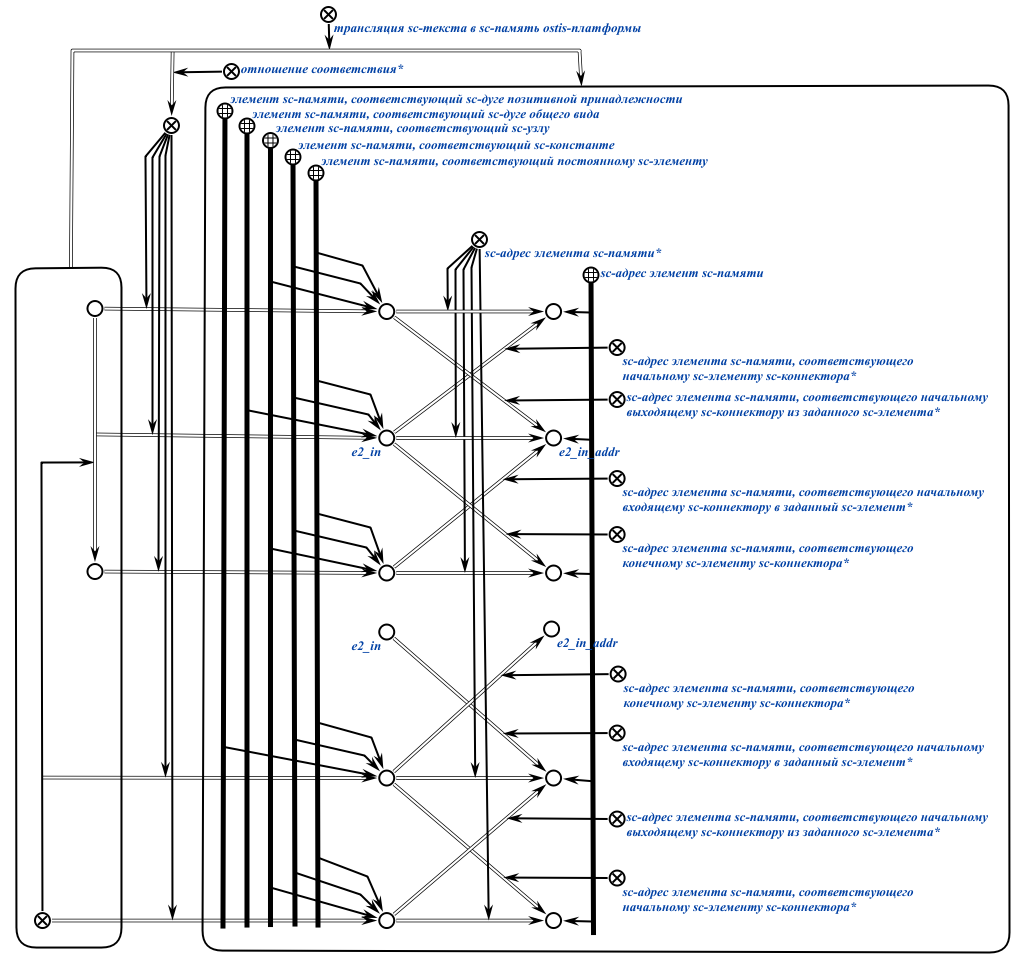
\includegraphics[scale=0.65]{author/part6/figures/sc_code_in_memory_representation.png}
    	%	\label{fig:sc_code_in_memory_representation}
    	%\end{figure*}
	}
    
    \end{scnsubstruct}
    
    \scnheader{SCin-код}
    \scntext{достоинства}{Описанная модель представления в текущей \textit{Реализации sc-памяти в ostis-платформы} \textit{синтаксических} и \textit{семантических классов sc-элементов} в виде \textit{синтаксических} и \textit{семантических классов элементов sc-памяти\scnsupergroupsign}, которые соответствуют первым, обладает рядом преимуществ:
    	\begin{itemize}
    		\item \textit{cинтаксические} и {семантические классы элементов sc-памяти\scnsupergroupsign} могут \uline{комбинироваться} между собой для получения более частных классов. С точки зрения программной реализации такая комбинация может быть представлена операцией \textit{битовое сложение*} \textit{классов элементов sc-памяти\scnsupergroupsign} (здесь, в спецификации на \textit{SC-коде} это можно сделать с помощью пересечения соответствующих классов). Так, например, \textit{битовое сложение*} классов \textit{элементов sc-памяти, соответствующих sc-узл}у и \textit{sc-константе} в результате образуют новый \textit{класс элементов sc-памяти\scnsupergroupsign} --- \textit{элемент sc-памяти, соответствующий константному sc-узлу}.
    		\item Числовые выражения некоторых классов могут совпадать. Это сделано для уменьшения размера \textit{элемента sc-памяти} за счет уменьшения максимального размера числового выражения класса этих \textit{элементов sc-памяти}. Конфликт в данном случае не возникает, поскольку такие классы не могут комбинироваться, например \textit{элемент sc-памяти, соответствующий sc-узлу ролевого отношения} и \textit{элемент sc-памяти, соответствующий sc-дуге нечеткой принадлежности}.
    		\item Важно отметить, что каждому из выделенных \textit{классов элементов sc-памяти} (кроме классов, получаемых путем комбинации других классов) однозначно соответствует порядковый номер бита в линейной памяти, что можно заметить, глядя на соответствующие числовые выражения этих классов. Это означает, что классы элементов не включаются друг в друга (хоть в спецификации это и не так), например, указание принадлежности к классу \textit{элементов sc-памяти, соответствующих sc-дуге позитивной принадлежности} не означает автоматическое указание принадлежности \textit{элементов sc-памяти, соответствующих sc-дуге принадлежности}. На уровне реализации это позволяет сделать операции комбинирования и сравнения меток более эффективными.
    	\end{itemize}
	}
    
    \scnheader{Реализация sc-памяти}
    \scntext{достоинства}{\textit{Реализация sc-памяти} учитывает технические аспекты реализации современных \textit{операционных систем}, что дает следующие достоинства:
    \begin{itemize}
    	\item Используемый подход адресации \textit{sc-элементов} позволяет загружать сегменты с диска в память, а также выгружать их обратно на диск в любой момент и при этом данная операция не требует дополнительных преобразований. Все содержимое из \textit{оперативной памяти} без изменений попадает на диск. Это дает возможность выгружать неиспользуемые сегменты на диск, что позволяет \textit{sc-памяти} абстрагироваться от имеющихся ресурсов \textit{оперативной памяти} и работать на любых ее объемах;
    	\item Максимальное количество хранимых \textit{sc-элементов} можно увеличивать путем расширения \textit{sc-адреса элемента sc-памяти}.
    \end{itemize}
    
    С точки зрения программной \textit{Реализации sc-памяти в ostis-платформе}, структура данных для хранения \textit{sc-узла} и \textit{sc-коннектора} остается остается та же, но в ней меняется список полей (компонентов). Кроме того, как можно заметить каждый \textit{элемент sc-памяти} (в том числе, \textit{элемент sc-памяти, соответствующий sc-дуге}) не хранит список \textit{sc-адресов} связанных с ним \textit{элементов sc-памяти}, а хранит \textit{sc-адреса} одного \textit{выходящего} и одного \textit{входящего элементов sc-памяти, соответствующих sc-коннекторам}, каждый из которых в свою очередь хранит \textit{sc-адреса следующего} и \textit{предыдущего элементов, соответствующих sc-коннекторам}, в списке выходящих и входящих \textit{элементов sc-памяти.} Все перечисленное позволяет:
    \begin{itemize}
    	\item сделать размер такой структуры фиксированным (в настоящее время 36 байт) и не зависящим от \textit{синтаксического класса} хранимого \textit{элемента в sc-памяти\scnsupergroupsign};
    	\item с минимальными временными затратами добавлять и удалять инцидентные элементы в и из программной структуры \textit{элемента sc-памяти} соответственно;
    	\item обеспечить возможность работы с sc-элементами без учета их синтаксического класса в случаях, когда это необходимо (например, при реализации поисковых запросов вида \scnqqi{Какие sc-элементы являются элементами данного множества}, \scnqqi{Какие sc-элементы непосредственно связаны с данным sc-элементом} и так далее);
    	\item обеспечить возможность доступа к \textit{элементу sc-памяти} за константное время;
    	\item обеспечить возможность помещения \textit{элемента sc-памяти} в процессорный кэш, что в свою очередь, позволяет ускорить обработку \textit{sc-конструкций}.
    \end{itemize}
	}
	\end{scnsubstruct}

    \scnheader{контекст процесса в рамках программной модели sc-памяти}
    \scnidtf{ScContext}
    \scnidtf{контекст процесса, выполняемого на уровне программной модели sc-памяти}
    \scnidtf{метаописание процесса в sc-памяти, выполняемого на уровне программной модели sc-памяти}
    \scnidtf{структура данных, содержащая метаинформацию о процессе, выполняемом в sc-памяти на уровне платформы}
    \scnrelto{класс компонентов}{Реализация sc-хранилища}
    \scntext{пояснение}{Каждому процессу, выполняемому в sc-памяти на уровне \textit{платформы интерпретации sc-моделей компьютерных систем} (и чаще всего соответствующего некоторому \textit{sc-агенту}, реализованному на уровне платформы) ставится в соответствие \textit{контекст процесса}, который является структурой данных, описывающей метаинформацию о данном процессе. На текущий момент контекст процесса содержит сведения об уровне доступа на чтение и запись для данного процесса (См. \textit{метка уровня доступа sc-элемента}).При вызове в рамках процесса любых функций (методов), связанных с доступом к хранимым в sc-памяти конструкциям одним из параметров обязательно является \textit{контекст процесса}.}
    \scnheader{блокировка sc-элемента в рамках программной модели sc-памяти}
    \scnidtf{ScLock}
    \scnrelto{класс компонентов}{Реализация sc-хранилища}
    \scnheader{подписка на событие в sc-памяти в рамках программной модели sc-памяти}
    \scnidtf{ScEvent}
    \scnidtf{структура данных, описывающая в рамках программной модели sc-памяти соответствие между классом событий в sc-памяти и действиями, которые должно быть совершены при возникновении в sc-памяти событий данного класса}
    \scnrelto{класс компонентов}{Реализация sc-хранилища}
    \scntext{пояснение}{Для того, чтобы обеспечить возможность создания sc-агентов в рамках \textit{платформы интерпретации sc-моделей компьютерных систем} реализована возможность создать подписку на событие, принадлежащее одному из классов \textit{элементарных событий в sc-памяти*} (см. Раздел \scnqqi{\textit{Предметная область и онтология темпоральных сущностей базы знаний ostis-системы}}), уточнив при этом sc-элемент, с которым должно быть связано событие данного класса (например, sc-элемент, для которого должна появиться входящая или исходящая sc-дуга). Подписка на событие представляет собой структуру данных, описывающую класс ожидаемых событий и функцию в программном коде, которая должна быть вызвана при возникновении данного события.Все подписки на события регистрируются в рамках таблицы событий. При любом изменении в sc-памяти происходит просмотр данной таблицы и запуск функций, соответствующих произошедшему событию.В текущей реализации обработка каждого события осуществляется в отдельном потоке операционной системы, при этом на уровне реализации задается параметр, описывающий число максимальных потоков, которые могут выполняться параллельно.Таким образом оказывается возможным реализовать sc-агенты, реагирующие на события в sc-памяти, а также при выполнении некоторого процесса в sc-памяти приостановить его работу и дождаться возникновения некоторого события (например, создать подзадачу некоторому коллективу sc-агентов и дождаться ее решения).}
    \scnheader{sc-итератор}
    \scnidtf{ScIterator}
    \scnrelto{класс компонентов}{Реализация sc-хранилища}
    \scntext{пояснение}{С функциональной точки зрения \textit{sc-итераторы} как часть \textit{Реализации sc-хранилища} представляют собой базовое средство доступа к конструкциям, хранимым в sc-памяти, которое позволяет осуществить чтение (просмотр) конструкций, изоморфных простейшим шаблонам --- \textit{трехэлементным sc-конструкциям} и \textit{пятиэлементным sc-конструкциям}.С точки зрения реализации \textit{sc-итератор} представляет собой структуру данных, которая соответствует определенному дополнительно уточняемому классу sc-конструкций и позволяет при помощи соответствующего набора функций последовательно осуществлять просмотр всех sc-конструкций данного класса, представленных в текущем состоянии sc-памяти (итерацию по sc-конструкциям).Каждому классу \textit{sc-итераторов} соответствует некоторый известный класс (шаблон, образец) \mbox{sc-конструкций}. При создании sc-итератора данный шаблон уточняется, то есть некоторым (как минимум одному) элементам шаблона ставится в соответствие конкретный заранее известный \textit{sc-элемент} (отправная точка при поиске), а другим элементам шаблона (тем, которые нужно найти) ставится в соответствие некоторый тип sc-элемента из числа типов, соответствующих \textit{меткам синтаксического типа sc-элемента}.Далее путем вызова соответствующей функции (или метода класса в ООП) осуществляется последовательный просмотр всех sc-конструкций, соответствующих полученному шаблону (с учетом указанных типов sc-элементов и заранее заданных известных sc-элементов), то есть \textit{sc-итератор} последовательно \scnqq{переключается} с одной конструкции на другую до тех пор, пока такие конструкции существуют. Проверка существования следующей конструкции проверяется непосредственно перед переключением. В общем случае конструкций, соответствующих указанному шаблону, может не существовать, в этом случае итерирование происходить не будет (будет 0 итераций).На каждой итерации в sc-итератор записываются sc-адреса sc-элементов, входящих в соответствующую sc-конструкцию, таким образом найденные элементы могут быть обработаны нужным образом в зависимости от задачи.}
    \scnsuperset{трехэлементный sc-итератор}
    \begin{scnindent}
        \scnrelfrom{класс sc-конструкций}{трехэлементная sc-конструкция}
    \end{scnindent}
    \scnsuperset{пятиэлементный sc-итератор}
    \begin{scnindent}
        \scnrelfrom{класс sc-конструкций}{пятиэлементная sc-конструкция}
        \scntext{примечание}{В настоящее время \textit{пятиэлементный sc-итератор} реализуется на основе \textit{трехэлементных sc-итераторов} и в этом смысле не является атомарным. Однако, введение \textit{пятиэлементных sc-итераторов} целесообразно с точки зрения удобства разработчика программ обработки \mbox{sc-конструкций}.}
    \end{scnindent}
    \scnheader{sc-шаблон}
    \scnidtf{ScTemplate}
    \scnidtf{структура данных в линейной памяти, описывающая обобщенную sc-структуру, которая в свою очередь может быть либо явно представлена sc-памяти, либо не представлена в ее текущем состоянии, но может быть представлена при необходимости}
    \scnrelto{класс компонентов}{Реализация sc-хранилища}
    \scntext{пояснение}{\textit{Sc-итераторы} позволяют осуществлять поиск только sc-конструкций простейшей конфигурации. Для реализации поиска sc-конструкций более сложной конфигурации, а также генерации сложных sc-конструкций используются \textit{sc-шаблоны}, на основе которых затем осуществляется поиск или генерация конструкций. \textit{Sc-шаблон} представляет собой структуру данных, соответствующую некоторой \textit{обобщенной структуре}, т.е. \textit{структуре}, содержащей \textit{sc-переменные}. При помощи соответствующего набора функций можно осуществлять
        \begin{scnitemize}
            \item поиск в текущем состоянии sc-памяти всех sc-конструкций, изоморфных заданному шаблону. В качестве параметров поиска можно указать значения для каких-либо из sc-переменных в составе шаблона. После осуществления поиска будет сформировано множество результатов поиска, каждый из которых представляет собой множество пар вида \scnqqi{sc-переменная из шаблона --- соответствующая ей sc-константа}. Данное множество может быть пустым (в текущем состоянии sc-памяти нет конструкций, изоморфных заданному образцу) или содержать один или более элементов. Подстановка значений sc-переменных может осуществляться как по sc-адресу, так и по системному sc-идентификатору;
            \item генерацию sc-конструкции, изоморфной заданному шаблону. Параметры и результаты генерации формируются так же, как в случае поиска, за исключением того, что в случае генерации результат всегда один и множество результатов не формируется.
        \end{scnitemize}
        Таким образом, каждый \textit{sc-шаблон} фактически задает множество шаблонов, формируемых путем указания значений для sc-переменных, входящих в исходный шаблон.Важно отметить, что \textit{sc-шаблон} представляет собой структуру данных в линейной памяти, соответствующую некоторой \textit{обобщенной структуре} в sc-памяти, но не саму эту \textit{обобщенную структуру}. Это означает, что sc-шаблон может быть автоматически сформирован на основе \textit{обобщенной структуры}, явно представленной в sc-памяти, а также сформирован на уровне программного кода путем вызова соответствующих функций (методов). Во втором случае \textit{sc-шаблон} будет существовать только в линейной памяти и соответствующая \textit{обобщенная структура} не будет явно представлена в sc-памяти. В этом случае подстановка значений sc-переменных будет возможна только по системному sc-идентификатору, поскольку sc-адресов у соответствующих элементов шаблона существовать не будет.}
    \scntext{примечание}{При поиске sc-конструкций, изоморфных заданному шаблону, крайне важно с точки зрения производительности с какого sc-элемента начинать поиск. Как известно, в общем случае задача поиска в графе представляет собой NP-полную задачу, однако поиск в sc-графе позволяет учитывать семантику обрабатываемой информации, что, в свою очередь, позволяет существенно снизить время поиска.Одним из возможных вариантов оптимизации алгоритма поиска, реализованным на данный момент, является упорядочение трехэлементных sc-конструкций, входящих в состав sc-шаблона, по очередности поиска по этим sc-конструкциям по критерию снижения числа возможных вариантов поиска, которые порождает та или иная трехэлементная sc-конструкция, содержащая sc-переменные. Так, в первую очередь при поиске выбираются те трехэлементные sc-конструкции, которые изначально содержат две sc-константы, затем те, которые изначально содержат одну sc-константу. После выполнения шага поиска приоритет sc-конструкций изменяется с учетом результатов, полученных на предыдущем шаге.Другой вариант оптимизации основывается на той особенности формализации в SC-коде, что в общем случае число sc-дуг, входящих в некоторый sc-элемент, как правило значительно меньше числа выходящих из него sc-дуг. Таким образом, целесообразным оказывается осуществлять поиск вначале по входящим sc-дугам.}
    \scntext{примечание}{Можно предположить, что возможности, предоставляемые \textit{sc-шаблонами} позволяют полностью исключить использование \textit{sc-итераторов}. Однако это не совсем так по следующим причинам:
        \begin{scnitemize}
            \item функции поиска и генерации по шаблону реализуются на основе sc-итераторов, как базового средства поиска sc-конструкций в рамках \textit{Реализации sc-хранилища}.
            \item \textit{sc-итераторы} дают возможность более гибко организовать процесс поиска с учетом семантики конкретных sc-элементов, участвующих в поиске. Так например, можно учесть тот факт, что для некоторых sc-элементов число входящих sc-дуг значительно меньше, чем выходящих (или наоборот) таким образом, при поиске конструкций, содержащих такие sc-элементы более эффективно начать перебор с тех участков, где дуг потенциально меньше.
        \end{scnitemize}
    }
	\end{scnsubstruct}

    \scnsegmentheader{Описание реализации подсистемы взаимодействия с внешней средой с использованием сетевых языков}
    \begin{scnsubstruct}
        \scnheader{Реализация подсистемы взаимодействия с внешней средой с использованием сетевых языков}
        \begin{scnrelfromlist}{компонент программной системы}
            \scnitem{Реализация подсистемы взаимодействия с внешней средой с использованием сетевых языков на основе языка JSON}
        \end{scnrelfromlist}
        \scntext{пояснение}{Взаимодействие программной модели sc-памяти с внешними ресурсами может осуществляться посредством специализированного программного интерфейса (API), однако этот вариант неудобен в большинстве случае, поскольку:
            \begin{scnitemize}
                \item поддерживается только для очень ограниченного набора языков программирования (С, С++);
                \item требует того, чтобы клиентское приложение, обращающееся к программной модели sc-памяти, фактически составляло с ней единое целое, таким образом исключается возможность построения распределенного коллектива ostis-систем;
                \item как следствие предыдущего пункта, исключается возможность параллельной работы с sc-памятью нескольких клиентских приложений.
            \end{scnitemize}
            Для того, чтобы обеспечить возможность удаленного доступа к sc-памяти не учитывая при этом языки программирования, с помощью которых реализовано конкретное клиентское приложение, было принято решение о реализации возможности доступа к sc-памяти с использованием универсального языка, не зависящего от средств реализации того или иного компонента или системы. В качестве такого языка был разработан строковый язык на базе языка JSON.}
        \scnstructheader{Описание подсистемы взаимодействия c sc-памятью на основе языка JSON}
        \begin{scnsubstruct}
            \scnheader{Реализация подсистемы взаимодействия c sc-памятью на основе языка JSON}
            \scntext{пояснение}{Реализация подсистемы взаимодействия c sc-памятью на основе языка JSON позволяет ostis-системам взаимодействовать с системами из внешней среды на основе общепринятого транспортного формата передачи данных JSON и предоставляет API для доступа к sc-памяти платформы интерпретации sc-моделей.}
            \begin{scnrelfromlist}{используемый язык программирования}
                \scnitem{C}
                \scnitem{C++}
                \scnitem{Python}
                \scnitem{TypeScript}
                \scnitem{C\#}
                \scnitem{Java}
            \end{scnrelfromlist}
            \begin{scnrelfromlist}{используемый язык}
                \scnitem{SC-JSON-код}
            \end{scnrelfromlist}
            \scnrelfrom{архитектура}{Клиент-серверная архитектура}
            \scnrelto{реализация}{Подсистема взаимодействия с sc-памятью на основе языка JSON}
            \begin{scnindent}
                \scnidtf{Подсистема взаимодействия с sc-памятью на основе формата JSON}
                \scnidtf{Подсистема взаимодействия с sc-памятью на основе транспортного формата передачи данных JSON}
                \scniselement{многократно используемый компонент ostis-систем}
                \scniselement{неатомарный многократно используемый компонент ostis-систем}
                \scniselement{зависимый многократно используемый компонент ostis-систем}
                \begin{scnrelfromlist}{автор}
                    \scnitem{Корончик Д. Н.}
                    \scnitem{Шункевич Д. В.}
                    \scnitem{Зотов Н. В.}
                    \scnitem{Загорский А. Г.}
                \end{scnrelfromlist}
                \scntext{пояснение}{Взаимодействие c sc-памятью обеспечивается с помощью передачи информации на \textit{\textbf{SC-JSON-коде}} и ведётся, с одной стороны, между сервером, являющегося частью ostis-системы, написанным на том же языке реализации этой ostis-системы и имеющим доступ к её sc-памяти, и с другой стороны множеством клиентом, которым известно о наличии сервера в пределах сети их использования.}
                \scntext{примечание}{Осмысленные фрагменты текстов \textit{\textbf{SC-JSON-кода}} представляют семантически корректную структуру сущностей и связей между ними.}
                \scntext{примечание}{С помощью подсистемы взаимодействия с sc-памятью на основе языка JSON можно взаимодействовать с ostis-системой на таком же множестве возможных операций, как и в случае, если бы взаимодействие происходило (непосредственно) напрямую, на том же языке реализации платформы интерпретации sc-моделей компьютерных систем. При этом результат работы отличается только скоростью обработки информации.}
                \begin{scnrelfromset}{декомпозиция программной системы}
                    \scnitem{Серверная система на основе Websocket, обеспечивающая доступ к sc-памяти платформы интерпретации sc-моделей при помощи команд SC-JSON-кода}
                    \scnitem{Множество клиентских систем, подключаемых и взаимодействующих с \textit{Серверной системой на основе Websocket, обеспечивающей доступ к sc-памяти платформы интерпретации sc-моделей при помощи команд SC-JSON-кода}}
                    \begin{scnindent}
                        \begin{scnrelfromset}{декомпозиция программной системы}
                            \scnitem{Клиентская система, подключаемая и взаимодействующая с \textit{SC-сервером}, реализованная на языке программирования Python}
                            \scnitem{Клиентская система, подключаемая и взаимодействующая с \textit{SC-сервером}, реализованная на языке программирования TypeScript}
                            \scnitem{Клиентская система, подключаемая и взаимодействующая с \textit{SC-сервером}, реализованная на языке программирования C\#}
                            \scnitem{Клиентская система, подключаемая и взаимодействующая с \textit{SC-сервером}, реализованная на языке программирования Java}
                        \end{scnrelfromset}
                    \end{scnindent}
                \end{scnrelfromset}
            \end{scnindent}
            \scnheader{SC-JSON-код}
            \scnidtf{Semantic JSON-code}
            \scnidtf{Semantic JavaScript Object Notation code}
            \scnidtf{Язык внешнего смыслового представления знаний для взаимодействия с ostis-системами на основе языка JSON}
            \scnidtf{Метаязык, являющийся подмножеством языка JSON и обеспечивающий внешнее представление и структуризацию \textit{sc-текстов}, используемых ostis-системой в процессе своего функционирования и взаимодействия со внешней средой.}
            \scntext{часто используемый неосновной внешний идентификатор sc-элемента}{sc-json-текст}
            \begin{scnindent}
                \scniselement{имя нарицательное}
            \end{scnindent}
            \scniselement{абстрактный язык}
            \scniselement{линейный язык}
            \scnsubset{JSON}
            \begin{scnrelfromlist}{автор}
                \scnitem{Зотов Н. В.}
                \scnitem{Корончик Д. Н.}
            \end{scnrelfromlist}
            \begin{scnrelfromvector}{принципы, лежащие в основе}
                \scnitem{Тексты, описываемые на языке внешнего представления знаний \textit{\textbf{SC-JSON-код}} представляют собой линейную структуру, представляемую в виде линейного строкового текста и состоящую из набора корректных осмысленных команд, записанных в виде \textit{sc-json-пар} вида \{отношение: объект\}, где отношением выступает знак квазибинарного отношения, состоящего из пар вида \{субъект: объект\}, где объектом выступает знак, обозначаемый предложением, включающее такие пары, а субъектом - sc-json-объекты: sc-json-литерал, sc-json-списки sc-json-объектов, sc-json-предложения, состоящие из sc-json-списков sc-json-объектов.}
                \scnitem{Тексты \textit{\textbf{SC-JSON-кода}} представляют собой sc-json-команды. Каждая команда представляет собой json-объект, в котором указываются уникальный идентификатор команды, тип этой команды и ее аргументы. C каждой командой ассоциируется ответ на эту команду. Ответ на команду представляет собой команду, в котором указываются идентификатор команды, ее статус (выполнена успешно/безуспешно) и результаты. Структура аргументов и результатов команды определяется типом команды. Для каждого ответа существует запрос.}
            \end{scnrelfromvector}
            \begin{scnrelfromlist}{достоинство}
                \scnfileitem{Язык JSON является общепринятым открытым форматом, для работы с которым существует большое количество библиотек для популярных языков программирования. Это, в свою очередь, упрощает реализацию клиента и сервера для протокола, построенного на базе \textit{\textbf{SC-JSON-код}}.}
                \scnfileitem{Реализация подсистемы взаимодействия со внешней средой на базе \textit{\textbf{SC-JSON-код}} не накладывает принципиальных ограничений на объем (длину) каждой команды, в отличие от других бинарных протоколов. Таким образом, появляется возможность использования неатомарных команд, позволяющих, например, за один акт пересылки такой команды по сети создать сразу несколько sc-элементов. Важными примерами таких команд являются \textit{команда создания sc-конструкции, изоморфной заданному sc-шаблону}, и \textit{команда поиска sc-конструкций, изоморфных заданному sc-шаблону}.}
            \end{scnrelfromlist}
            \scntext{примечание}{Можно сказать, что язык на базе JSON является следующим шагом на пути к созданию мощного и универсального языка запросов, аналогичного языку SQL для реляционных баз данных и предназначенному для работы с sc-памятью. Следующий шагом станет реализация такого протокола на основе одного из стандартов внешнего отображения sc-конструкций, например, \textit{SCs-кода}, что, в свою очередь, позволит передавать в качестве команд целые программы обработки sc-конструкций, например на языке SCP.}
            \scnstructheader{Синтаксис SC-JSON-кода}
            \begin{scnsubstruct}
                \scnheader{Синтаксис SC-JSON-кода}
                \scntext{примечание}{\textit{Синтаксис SC-JSON-кода} задается: (1) \textit{Алфавитом SC-JSON-кода}, (2) Грамматикой SC-JSON-кода}
                \scnrelto{синтаксис}{SC-JSON-код}
                \scnstructheader{Синтаксическая классификация элементов SC-JSON-кода}
                \begin{scnsubstruct}
                    \scnstructheader{SC-JSON-код}
                    \scnrelto{семейство подмножеств}{sc-json-предложение}
                    \begin{scnindent}
                        \scnsubset{json-список json-пар}
                        \scnrelto{семейство подмножеств}{sc-json-пара*}
                        \begin{scnindent}
                            \begin{scnreltovector}{декартово произведение}
                                \scnitem{sc-json-строка}
                                \scnitem{sc-json-объект}
                                \begin{scnindent}
                                    \begin{scnrelfromset}{разбиение}
                                        \scnitem{sc-json-cписок}
                                        \scnitem{sc-json-пара}
                                        \scnitem{sc-json-литерал}
                                        \begin{scnindent}
                                            \begin{scnrelfromset}{разбиение}
                                                \scnitem{sc-json-строка}
                                                \scnitem{sc-json-число}
                                            \end{scnrelfromset}
                                        \end{scnindent}
                                    \end{scnrelfromset}
                                \end{scnindent}
                            \end{scnreltovector}
                        \end{scnindent}
                        \begin{scnrelfromset}{разбиение}
                            \scnitem{команда на SC-JSON-коде}
                            \scnitem{ответ на команду на SC-JSON-коде}
                        \end{scnrelfromset}
                    \end{scnindent}
                \end{scnsubstruct}
                \scnsourcecomment{Завершили представление \textit{Синтаксической классификации элементов SC-JSON-кода}}
                \scnheader{Алфавит SC-JSON-кода\scnsupergroupsign}
                \scnidtf{Множество всех возможных символов в SC-JSON-коде}
                \scntext{пояснение}{Поскольку SC-JSON-код является линейным строковым языком представления знаний, то его алфавит включает объединение алфавитов всех языков, тексты на которых могут представлять внешние идентификаторы и/или содержимое файлов ostis-системы, множество всех цифр и множество всех других специальных символов.}
                \scnrelto{алфавит}{SC-JSON-код}
                \scntext{примечание}{Последовательности знаков алфавита могут образовывать sc-json ключевые слова, sc-json-пары, sc-json-предложения из sc-json-пар и sc-json-тексты из sc-json-предложений.}
                \scnheader{SC-JSON-код}
                \begin{scnrelfromlist}{синтаксические правила}
                    \scnfileitem{Каждое правило \textit{Грамматики SC-JSON-кода} описывает корректный с точки зрения \textit{Синтаксиса SC-JSON-кода} порядок sc-json-объектов в sc-json-предложении. Совокупность правил \textit{Грамматики SC-JSON-кода} описывает корректный с точки зрения \textit{Синтаксиса SC-JSON-кода} порядок sc-json-предложений в sc-json-тексте.}
                    \scnfileitem{Каждое sc-json-предложение является sc-json-списком, состоящим из sc-json-пар и представляет собой команду или ответ на эту команду.}
                    \scnfileitem{Каждое \textit{команда (ответ на команду) на SC-JSON-коде} состоит из заголовка, включающего sc-json-пары описания самой команды (ответа на команду), и сообщения, различного для каждого класса команд (ответов на команды). Сообщение \textit{команды (ответа на команду) на SC-JSON-коде} обычно представляет собой список sc-json-объектов и может не ограничиваться по мощности.}
                    \scnfileitem{Каждая sc-json-пара состоит из двух элементов: ключевого слова и некоторого другого sc-json-объекта, ассоциируемого с этим ключевым словом. Набор ключевых слов в sc-json-парах определяется конкретным классом \textit{команд (ответов на команды) на SC-JSON-коде}. Sc-json-пара начинается знаком открывающейся фигурной скобки \scnqq{\{} и заканчивается знаком закрывающейся фигурной скобки \scnqq{\}}. Ключевое слово и sc-json-объект, ассоциируемый с ним, разделяются при помощи знака двоеточия \scnqq{:}.}
                    \scnfileitem{Sc-json-строки, записанные в sc-json-текстах, начинаются и заканчиваются знаком двух ковычек \textquotedblleft.}
                    \scnfileitem{Sc-json-списки, состоящие не из sc-json-пар, начинаются знаком открывающейся квадратной скобки \scnqq{} и заканчиваются знаком закрывающейся квадратной скобки \scnqq{}. Sc-json-объекты в sc-json-списках разделяются запятыми \scnqq{,}.}
                \end{scnrelfromlist}
                \scnheader{Грамматика SC-JSON-кода}
                \scnidtf{Множество всех возможных правил, используемых при построении команд и ответов на них на SC-JSON-коде}
                \scntext{пояснение}{Каждой команде \textit{SC-JSON-кода} однозначно соответствует правило грамматики \textit{SC-JSON-кода}.}
                \scnrelto{грамматика}{SC-JSON-код}
                \scntext{пояснение}{Правила \textit{Грамматики SC-JSON-кода} позволяют правильно составить команду на SC-JSON-коде. Каждое правило грамматики \textit{SC-JSON-кода} представляется в виде правила на \textit{Языке описания грамматик ANTLR} и его интерпретации на естественном языке.}
                \scnhaselementrole{ключевой sc-элемент}{Правило, задающее синтаксис \textit{команд на SC-JSON-коде}}
                \begin{scnindent}
                    \scnrelboth{семантическая эквивалентность}{\scnfileimage[20em]{Contents/part_platform/images/command.png}}
                    \begin{scnindent}
                        \scniselement{Язык описания грамматики языков ANTLR}
                        \scntext{интерпретация}{Класс \textit{команд на SC-JSON-коде} включает \textit{команду создания sc-элементов}, \textit{команду получения соответствующих типов sc-элементов}, \textit{команду удаления sc-элементов}, \textit{команду обработки ключевых sc-элементов}, \textit{команду обработки содержимого файлов ostis-системы}, \textit{команду поиска sc-конструкций, изоморфных заданному sc-шаблону}, \textit{команду генерации sc-конструкции, изоморфной заданному sc-шаблону}, и \textit{команду обработки sc-событий}. В \textit{команду на SC-JSON-коде} включаются идентификатор этой команды, тип и сообщение.}
                    \end{scnindent}
                    \scnrelto{синтаксическое правило}{команда на SC-JSON-коде}
                \end{scnindent}
                \scnhaselementrole{ключевой sc-элемент}{Правило, задающее синтаксис \textit{ответа на команду на SC-JSON-коде}}
                \begin{scnindent}
                    \scnrelboth{семантическая эквивалентность}{\scnfileimage[20em]{Contents/part_platform/images/command_answer.png}}
                    \begin{scnindent}
                        \scniselement{Язык описания грамматики языков ANTLR}
                        \scntext{интерпретация}{Класс \textit{ответов на команды на SC-JSON-коде} включает \textit{ответ на команду создания sc-элементов}, \textit{ответ на команду получения соответствующих типов sc-элементов}, \textit{ответ на команду удаления sc-элементов}, \textit{ответ на команду обработки ключевых sc-элементов}, \textit{ответ на команду обработки содержимого файлов ostis-системы}, \textit{ответ на команду поиска sc-конструкций, изоморфных заданному sc-шаблону}, \textit{ответ на команду генерации sc-конструкции, изоморфной заданному sc-шаблону}, и \textit{ответ на команду обработки sc-событий}. В \textit{ответ на команду на SC-JSON-коде} включаются идентификатор соответствующей команды, статус обработки ответа и ответное сообщение.}
                    \end{scnindent}
                    \scnrelto{синтаксическое правило}{ответ на команду на SC-JSON-коде}
                \end{scnindent}
                \scnhaselement{Правило, задающее синтаксис \textit{команды создания sc-элементов}}
                \begin{scnindent}
                    \scnrelboth{семантическая эквивалентность}{\scnfileimage[20em]{Contents/part_platform/images/create_elements_command.pdf}}
                    \begin{scnindent}
                        \scniselement{Язык описания грамматики языков ANTLR}
                        \scntext{интерпретация}{В сообщении \textit{команды создания sc-элементов} представляется список описаний создаваемых sc-элементов. Такими sc-элементами могут быть sc-узел, sc-дуга, sc-ребро или файл ostis-системы. Тип sc-элемента указывается в паре с ключевым словом \scnqq{el}: для sc-узла sc-json-тип элемент представляется как \scnqq{node}, для sc-дуги и sc-ребра - \scnqq{edge}, для файла ostis-системы - \scnqq{link}. Метки типов sc-элементов уточняются в соответствующих им описаниях в сообщении команды в паре с ключевым словом \scnqq{type}. Если создаваемым sc-элементом является файл ostis-системы, то дополнительно указывается содержимое этого файла ostis-системы в паре с ключевым словом \scnqq{content}, если создаваемым sc-элементом является sc-дуга или sc-ребро, то указываются описания sc-элементов, из которых они выходят, и sc-элементов, в которые они входят. Описание таких sc-элементов состоят из двух пар: первая пара указывает на способ ассоциации с sc-элементом и представляется как \scnqq{addr} или \scnqq{idtf} или \scnqq{ref} в паре с ключевым словом \scnqq{type}, вторая пара - то, по чему происходит ассоциация с этим sc-элементом: его хэшу, системному идентификатору или номеру в массиве создаваемых sc-элементов - в паре с ключевым словом \scnqq{value}.}
                    \end{scnindent}
                    \scnrelto{синтаксическое правило}{команда создания sc-элементов}
                \end{scnindent}
                \scnhaselement{Правило, задающее синтаксис \textit{ответа на команду создания sc-элементов}}
                \begin{scnindent}
                    \scnrelboth{семантическая эквивалентность}{\scnfileimage[20em]{Contents/part_platform/images/create_elements_command_answer.png}}
                    \begin{scnindent}
                        \scniselement{Язык описания грамматики языков ANTLR}
                        \scntext{интерпретация}{Сообщением \textit{ответа на команду создания sc-элементов} является список хэшей созданных sc-элементов, соответствующих описаниям \textit{команды создания sc-элементов} со статусом 1, в случае успешной обработки команды.}
                    \end{scnindent}
                    \scnrelto{синтаксическое правило}{ответ на команду создания sc-элементов}
                \end{scnindent}
                \scnhaselement{Правило, задающее синтаксис \textit{команды создания sc-элементов по фрагменту SCs-текста}}
                \begin{scnindent}
                    \scnrelboth{семантическая эквивалентность}{\scnfileimage[20em]{Contents/part_platform/images/create_elements_by_scs_command.png}
                    }
                    \begin{scnindent}
                        \scniselement{Язык описания грамматики языков ANTLR}
                        \scntext{интерпретация}{В списке описаний создаваемых sc-элементов сообщения этой команды вместо описания создаваемого отдельного sc-элемента указывается фрагмент SCs-текста.}
                    \end{scnindent}
                    \scnrelto{синтаксическое правило}{команда создания sc-элементов по фрагменту SCs-текста}
                \end{scnindent}
                \scnhaselement{Правило, задающее синтаксис \textit{ответа на команду создания sc-элементов по фрагменту SCs-текста}}
                \begin{scnindent}
                    \scnrelboth{семантическая эквивалентность}{\scnfileimage[10em]{Contents/part_platform/images/create_elements_by_scs_command_answer.png}}
                    \begin{scnindent}
                        \scniselement{Язык описания грамматики языков ANTLR}
                        \scntext{интерпретация}{Сообщением \textit{ответа на команду создания sc-элементов} является список результатов обработки переданных SCs-текстов. Нулевой статус говорит о том, что обработка соотвествующего SCs-текста завершилась безуспешно.}
                    \end{scnindent}
                    \scnrelto{синтаксическое правило}{ответ на команду создания sc-элементов по фрагменту SCs-текста}
                \end{scnindent}
                \scnhaselement{Правило, задающее синтаксис \textit{команды получения соответствующих типов sc-элементов}}
                \begin{scnindent}
                    \scnrelboth{семантическая эквивалентность}{\scnfileimage[20em]{Contents/part_platform/images/check_elements_command.png}}
                    \begin{scnindent}
                        \scniselement{Язык описания грамматики языков ANTLR}
                        \scntext{интерпретация}{Сообщением \textit{команды получения соответствующих типов sc-элементов} является списком хэшей sc-элементов, у которых необходимо получить синтаксические типы.}
                    \end{scnindent}
                    \scnrelto{синтаксическое правило}{команда получения соответствующих типов sc-элементов}
                \end{scnindent}
                \scnhaselement{Правило, задающее синтаксис \textit{ответа на команду получения соответствующих типов sc-элементов}}
                \begin{scnindent}
                    \scnrelboth{семантическая эквивалентность}{\scnfileimage[20em]{Contents/part_platform/images/check_elements_command_answer.png}}
                    \begin{scnindent}
                        \scniselement{Язык описания грамматики языков ANTLR}
                        \scntext{интерпретация}{Сообщением \textit{ответа на команду получения соответствующих типов sc-элементов} является список типов проверенных sc-элементов, соответствующих описаниям \textit{команды получения соответствующих типов sc-элементов} со статусом 1, в случае успешной обработки команды.}
                    \end{scnindent}
                    \scnrelto{синтаксическое правило}{ответ на команду получения соответствующих типов sc-элементов}
                \end{scnindent}
                \scnhaselement{Правило, задающее синтаксис \textit{команды удаления sc-элементов}}
                \begin{scnindent}
                    \scnrelboth{семантическая эквивалентность}{\scnfileimage[20em]{Contents/part_platform/images/delete_elements_command.png}
                    }
                    \begin{scnindent}
                        \scniselement{Язык описания грамматики языков ANTLR}
                        \scntext{интерпретация}{Сообщением \textit{команды удаления sc-элементов} является список хэшей sc-элементов, которые необходимо удалить из sc-памяти.}
                    \end{scnindent}
                    \scnrelto{синтаксическое правило}{команда удаления sc-элементов}
                \end{scnindent}
                \scnhaselement{Правило, задающее синтаксис \textit{ответа на команду удаления sc-элементов}}
                \begin{scnindent}
                    \scnrelboth{семантическая эквивалентность}{\scnfileimage[20em]{Contents/part_platform/images/delete_elements_command_answer.png}}
                    \begin{scnindent}
                        \scniselement{Язык описания грамматики языков ANTLR}
                        \scntext{интерпретация}{Сообщение \textit{ответа на команду удаления sc-элементов} является пустым со статусом 1, в случае успешной обработки команды.}
                    \end{scnindent}
                    \scnrelto{синтаксическое правило}{ответ на команду удаления sc-элементов}
                \end{scnindent}
                \scnhaselement{Правило, задающее синтаксис \textit{команды обработки ключевых sc-элементов}}
                \begin{scnindent}
                    \scnrelboth{семантическая эквивалентность}{\scnfileimage[20em]{Contents/part_platform/images/handle_keynodes_command.png}}
                    \begin{scnindent}
                        \scniselement{Язык описания грамматики языков ANTLR}
                        \scntext{интерпретация}{Сообщение \textit{команды обработки ключевых sc-элементов} может включать описание ключевых sc-элементов, которые необходимо найти и/или разрешить по их идентификаторам. Такое деление осуществляется с помощью подкоманд, содержащихся в сообщении команды. Идентификаторами подкоманд могут быть \scnqq{find} и \scnqq{resolve} соответственно, стоящие в паре с ключевым словом \scnqq{command}. Описание искомого sc-элемента команды \scnqq{find} включает системный идентификатор sc-элемента, по которому необходимо найти этот sc-элемент, стоящий в паре с ключевым словом \scnqq{idtf}. Описание разрешаемого sc-элемента команды \scnqq{resolve} включает системный идентификатор sc-элемента, по которому необходимо найти этот sc-элемент, либо в случае безуспешного поиска создать sc-элемент некоторого типа, указанного в его описании в паре с ключевым словом \scnqq{elType}, и установить для него системный идентификатор, по которому была произведена попытка найти другой sc-элемент.}
                    \end{scnindent}
                    \scnrelto{синтаксическое правило}{команда обработки ключевых sc-элементов}
                \end{scnindent}
                \scnhaselement{Правило, задающее синтаксис \textit{ответа на команду обработки ключевых sc-элементов}}
                \begin{scnindent}
                    \scnrelboth{семантическая эквивалентность}{\scnfileimage[20em]{Contents/part_platform/images/handle_keynodes_command_answer.png}}
                    \begin{scnindent}
                        \scniselement{Язык описания грамматики языков ANTLR}
                        \scntext{интерпретация}{Сообщением \textit{ответа на команду обработки ключевых sc-элементов} является список хэшей sc-элементов, соответствующих описаниям \textit{команды обработки ключевых sc-элементов} со статусом 1, в случае успешной обработки команды.}
                    \end{scnindent}
                    \scnrelto{синтаксическое правило}{ответ на команду обработки ключевых sc-элементов}
                \end{scnindent}
                \scnhaselement{Правило, задающее синтаксис \textit{команды обработки содержимого файлов ostis-системы}}
                \begin{scnindent}
                    \scnrelboth{семантическая эквивалентность}{\scnfileimage[10em]{Contents/part_platform/images/handle_link_contents_command.png}}
                    \begin{scnindent}
                        \scniselement{Язык описания грамматики языков ANTLR}
                        \scntext{интерпретация}{Сообщение \textit{команды обработки содержимого файлов ostis-системы} может включать описание ключевых файлов ostis-системы, которые необходимо найти по их содержимому или части этого содержимого, для которых необходимо установить содержимое разрешить и/или у которых необходимо получить содержимое. Как и в \textit{Правиле, задающее синтаксис команды обработки ключевых sc-элементов} деление осуществляется с помощью подкоманд, содержащихся в сообщении команды. Идентификаторами подкоманд могут быть \scnqq{find}, \scnqq{find\_by\_substr}, \scnqq{set} и \scnqq{get} соответственно, стоящие в паре с ключевым словом \scnqq{command}. В описаниях команд \scnqq{set} и \scnqq{get} указывается хэш файла ostis-системы в паре с ключевым словом \scnqq{addr}. В описаниях команд \scnqq{set}, \scnqq{find} и \scnqq{find\_by\_substr} указывается содержимое файла ostis-системы в паре с ключевым словом \scnqq{data}. Дополнительно в описании подкоманды \scnqq{set} указывается тип устанавливаемого содержимого файла ostis-системы.}
                    \end{scnindent}
                    \scnrelto{синтаксическое правило}{команда обработки содержимого файлов ostis-системы}
                \end{scnindent}
                \scnhaselement{Правило, задающее синтаксис \textit{ответа на команду обработки содержимого файлов ostis-системы}}
                \begin{scnindent}
                    \scnrelboth{семантическая эквивалентность}{\scnfileimage[60em]{Contents/part_platform/images/handle_link_contents_command_answer.png}
                    }
                    \begin{scnindent}
                        \scniselement{Язык описания грамматики языков ANTLR}
                        \scntext{интерпретация}{Сообщением \textit{ответа на команду обработки содержимого файлов ostis-системы} является список, состоящий из булевого результата установки содержимого в файл ostis-системы и/или найденных файлов ostis-системы по их содержимому и/или описания полученного содержимого файлов ostis-системы, соответствующих описаниям \textit{команды обработки содержимого файлов ostis-системы} со статусом 1, в случае успешной обработки команды.}
                    \end{scnindent}
                    \scnrelto{синтаксическое правило}{ответ на команду обработки содержимого файлов ostis-системы}
                \end{scnindent}
                \scnhaselement{Правило, задающее синтаксис \textit{команды поиска sc-конструкций, изоморфных заданному sc-шаблону}}
                \begin{scnindent}
                    \scnrelboth{семантическая эквивалентность}{\scnfileimage[10em]{Contents/part_platform/images/search_template_command.png}}
                    \begin{scnindent}
                        \scniselement{Язык описания грамматики языков ANTLR}
                        \scnsubset{Правило, задающее синтаксис сообщения \textit{команды поиска sc-конструкций, изоморфных заданному sc-шаблону}, и \textit{команды генерации sc-конструкции, изоморфной заданному sc-шаблону}}
                        \scntext{интерпретация}{\textit{Правило, задающее синтаксис команды поиска sc-конструкций, изоморфных заданному sc-шаблону} включает \textit{Правило, задающее синтаксис сообщения \textit{команды поиска sc-конструкций, изоморфных заданному sc-шаблону,} и \textit{команды генерации sc-конструкции, изоморфной заданному sc-шаблону}} и описывает команду поиска sc-конструкций по сформированному этой командой sc-шаблону (см. \textit{Правило, задающее синтаксис сообщения \textit{команды поиска sc-конструкций, изоморфных заданному sc-шаблону,} и \textit{команды генерации sc-конструкции, изоморфной заданному sc-шаблону}}).}
                    \end{scnindent}
                    \scnrelto{синтаксическое правило}{команда поиска sc-конструкций, изоморфных заданному sc-шаблону}
                \end{scnindent}
                \scnhaselement{Правило, задающее синтаксис \textit{ответа на команду поиска sc-конструкций, изоморфных заданному sc-шаблону}}
                \begin{scnindent}
                    \scnrelboth{семантическая эквивалентность}{\scnfileimage[15em]{Contents/part_platform/images/search_template_command_answer.png}}
                    \begin{scnindent}
                        \scniselement{Язык описания грамматики языков ANTLR}
                        \scntext{интерпретация}{Сообщение \textit{ответа на команду поиска sc-конструкций, изоморфных заданному sc-шаблону} состоит из списка найденных sc-конструкций и отображения псевдонимов sc-элементов на их позиции в тройках sc-шаблона. Ответ имеет статус 1, в случае успешной обработки команды.}
                    \end{scnindent}
                    \scnrelto{синтаксическое правило}{ответ на команду поиска sc-конструкций, изоморфных заданному sc-шаблону}
                \end{scnindent}
                \scnhaselement{Правило, задающее синтаксис \textit{команды создания sc-конструкции, изоморфной заданному sc-шаблону}}
                \begin{scnindent}
                    \scnrelboth{семантическая эквивалентность}{\scnfileimage[20em]{Contents/part_platform/images/generate_template_command.png}}
                    \begin{scnindent}
                        \scniselement{Язык описания грамматики языков ANTLR}
                        \scnsubset{Правило, задающее синтаксис сообщения \textit{команды поиска sc-конструкций, изоморфных заданному sc-шаблону,} и \textit{команды генерации sc-конструкции, изоморфной заданному sc-шаблону}}
                        \scntext{интерпретация}{\textit{Правило, задающее синтаксис команды создания sc-конструкции, изоморфной заданному sc-шаблону} включает \textit{Правило, задающее синтаксис сообщения \textit{команды поиска sc-конструкций, изоморфных заданному sc-шаблону,} и \textit{команды генерации sc-конструкции, изоморфной заданному sc-шаблону}} и описывает команду создания sc-конструкции по сформированному этой командой sc-шаблону (см. \textit{Правило, задающее синтаксис сообщения \textit{команды поиска sc-конструкций, изоморфных заданному sc-шаблону,} и \textit{команды генерации sc-конструкции, изоморфной заданному sc-шаблону}}).}
                    \end{scnindent}
                    \scnrelto{синтаксическое правило}{команда создания sc-конструкции, изоморфной заданному sc-шаблону}
                \end{scnindent}
                \scnhaselement{Правило, задающее синтаксис \textit{ответа на команду создания sc-конструкции, изоморфной заданному sc-шаблону}}
                \begin{scnindent}
                    \scnrelboth{семантическая эквивалентность}{\scnfileimage[20em]{Contents/part_platform/images/generate_template_command_answer.png}}
                    \begin{scnindent}
                        \scniselement{Язык описания грамматики языков ANTLR}
                        \scntext{интерпретация}{Сообщение \textit{ответа на команду создания sc-конструкции, изоморфной заданному sc-шаблону} состоит из списка найденных sc-конструкций и отображения псевдонимов sc-элементов на их позиции в тройках sc-шаблона. Ответ имеет статус 1, в случае успешной обработки команды.}
                    \end{scnindent}
                    \scnrelto{синтаксическое правило}{ответ на команду создания sc-конструкции, изоморфной заданному sc-шаблону}
                \end{scnindent}
                \scnhaselement{Правило, задающее синтаксис сообщения \textit{команды поиска sc-конструкций, изоморфных заданному sc-шаблону,} и \textit{команды создания sc-конструкции, изоморфной заданному sc-шаблону}}
                \begin{scnindent}
                    \scnrelboth{семантическая эквивалентность}{\scnfileimage[20em]{Contents/part_platform/images/template_message_command.png}}
                    \begin{scnindent}
                        \scniselement{Язык описания грамматики языков ANTLR}
                        \scntext{интерпретация}{Сообщения \textit{команды поиска sc-конструкций, изоморфных заданному sc-шаблону,} и \textit{команды создания sc-конструкции, изоморфной заданному sc-шаблону} включают описание троек, необходимых для создания sc-шаблона поиска или генерации изоморфных sc-конструкций. Описание каждой тройки sc-шаблона включает описание sc-элементов этой тройки. Описания первого и третьего sc-элементов тройки должны всегда содержать хэш или тип в паре с ключевым словом \scnqq{value}. Если выбран тип, то в паре с ключевым словом \scnqq{type} указывается \scnqq{type}, если - хэш, то - \scnqq{addr}. Вторым sc-элементом тройки должна быть дуга, для которой всегда указывается тип в паре с ключевым словом \scnqq{value}. Для каждого sc-элемента тройки может указываться псевдоним в паре с \scnqq{alias}. Псевдоним представляет собой строку и может быть использован для ассоциации с sc-элементами в других тройках sc-шаблона, либо ассоциации со значениями переменных sc-шаблона, которые указываются в списке под ключевым словом \scnqq{params} и могут представлять собой либо хэш sc-элемента, либо его системный идентификатор. Таким образом, в некоторых случаях может отсутствовать необходимость указания хэша или типа sc-элемента. Также вместо списка описаний троек sc-шаблона, может указываться хэш или системный идентификатор sc-структуры, хранящейся в sc-памяти. хэш и системный идентификатор указываются в паре с ключевым словом \scnqq{value}.}
                    \end{scnindent}
                \end{scnindent}
                \scnhaselement{Правило, задающее синтаксис \textit{команды обработки sc-событий}}
                \begin{scnindent}
                    \scnrelboth{семантическая эквивалентность}{\scnfileimage[20em]{Contents/part_platform/images/handle_events_command.png}}
                    \begin{scnindent}
                        \scniselement{Язык описания грамматики языков ANTLR}
                        \scntext{интерпретация}{Сообщение \textit{команды обработки sc-событий} может включать описание sc-элементов, по котором необходимо зарегистрировать или разрегистрировать sc-события. Идентификаторами подкоманд в описании команды могут быть \scnqq{create} и \scnqq{delete} соответственно, стоящие в паре с ключевым словом \scnqq{command}. Описание команды регистрации sс-cобытий \scnqq{create} представляет собой список описаний типов sc-событий и sc-элементов, по которым необходимо зарегистрировать sc-события. Описания sc-элементов включают хэши этих sc-элементов в парах с ключевым словом \scnqq{addr}. Описание команды разрегистрации sc-событий представляет собой список позиций sc-событий в очереди sc-событий, которые необходимо удалить из этой очереди sc-событий.}
                    \end{scnindent}
                    \scnsuperset{Правило, задающее синтаксис типов sc-событий}
                    \begin{scnindent}
                        \scnrelboth{семантическая эквивалентность}{\scnfileimage[10em]{Contents/part_platform/images/sc_event_types.png}}
                        \begin{scnindent}
                            \scniselement{Язык описания грамматики языков ANTLR}
                            \scntext{интерпретация}{Sc-событиями могут быть \textit{sc-события добавления выходящей дуги из sc-элемента (add\_outgoing\_edge)}, \textit{sc-события добавления входящей дуги в sc-элемент (add\_ingoing\_edge)}, \textit{sc-события удаления выходящей дуги из sc-элемента (remove\_outgoing\_edge)}, \textit{sc-события удаления входящей дуги в sc-элемент (remove\_ingoing\_edge)}, \textit{sc-события изменения содержимого файла ostis-системы (content\_change)} и \textit{sc-события удаления sc-элемента (delete\_element)}.}
                        \end{scnindent}
                    \end{scnindent}
                    \scnrelto{синтаксическое правило}{команда обработки sc-событий}
                \end{scnindent}
                \scnhaselement{Правило, задающее синтаксис \textit{ответа на команду обработки sc-событий}}
                \begin{scnindent}
                    \scnrelboth{семантическая эквивалентность}{\scnfileimage[30em]{Contents/part_platform/images/handle_events_command_answer.png}}
                    \begin{scnindent}
                        \scniselement{Язык описания грамматики языков ANTLR}
                        \scntext{интерпретация}{Сообщение \textit{ответа на команду обработки sc-событий} состоит из позиций зарегистрированных sc-событий в очереди. Успешным результатом \textit{команды обработки sc-событий} является статус 1.}
                    \end{scnindent}
                    \scnrelto{синтаксическое правило}{ответ на команду обработки sc-событий}
                \end{scnindent}
                \scnhaselement{Правило, задающее синтаксис \textit{ответа инициализации sc-события}}
                \begin{scnindent}
                    \scnrelboth{семантическая эквивалентность}{\scnfileimage[20em]{Contents/part_platform/images/init_event_command_answer.png}}
                    \begin{scnindent}
                        \scniselement{Язык описания грамматики языков ANTLR}
                        \scntext{интерпретация}{\textit{Ответ инициализации sc-события} возникает тогда и только тогда, когда в sc-памяти инициализируется соответствующее sc-событие. \textit{Ответ инициализации sc-события} всегда отсылается той клиентской системе, которая зарегистрировала это sc-событие. В сообщение \textit{ответа инициализации sc-события} включаются хэши тех sc-элементов, которые связаны с зарегистрированным sc-событием. Таким образом, если было зарегистрировано sc-событие выходящей sc-дуги, то в списке сообщения \textit{ответа инициализации sc-события} будут находится хэши трёх sc-элементов: хэш sc-элемента, который был подписан на sc-событие, хэш добавленной выходящей из него sc-дуги и хэш sc-элемента, являющегося концом этой sc-дуги.}
                    \end{scnindent}
                    \scnrelto{синтаксическое правило}{ответ инициализации sc-события}
                \end{scnindent}
                \scnhaselement{Правило, задающее синтаксис \textit{синтаксических типов sc-элементов}}
                \begin{scnindent}
                    \scnrelboth{семантическая эквивалентность}{\scnfileimage[10em]{Contents/part_platform/images/sc_addr_types.png}}
                    \begin{scnindent}
                        \scniselement{Язык описания грамматики языков ANTLR}
                        \scntext{интерпретация}{\textit{Правило, задающее синтаксис синтаксических типов sc-элементов} включает \textit{Правило, задающее синтаксис синтаксических типов sc-узлов}, \textit{Правило, задающее синтаксис синтаксических типов sc-дуг}, \textit{Правило, задающее синтаксис синтаксических типов файлов ostis-системы}. Синтаксические типы sc-элементов представляются в виде целого числа и соответствуют программным синтаксическим типам, представляемым в sc-памяти.}
                    \end{scnindent}
                    \scntext{примечание}{На данный момент форма представления синтаксического типа sc-элемента зависит от того, как располагаются биты в маске sc-элемента. Следующим шагом в развитии \textit{SC-JSON-кода} и его грамматики могли быть стать устранение такой зависимости и переход к представлению синтаксических типов в виде строковых литералов, интерпретируемых \textit{Серверной системы на основе Websocket, обеспечивающей доступ к sc-памяти платформы интерпретации sc-моделей при помощи команд SC-JSON-кода}.}
                \end{scnindent}
                \scnhaselement{Правило, задающее синтаксис \textit{синтаксических типов sc-узлов}}
                \begin{scnindent}
                    \scnrelboth{семантическая эквивалентность}{\scnfileimage[20em]{Contents/part_platform/images/sc_node_types.png}}
                    \begin{scnindent}
                        \scniselement{Язык описания грамматики языков ANTLR}
                        \scntext{интерпретация}{\textit{Правило, задающее синтаксис синтаксических типов sc-узлов} описывает возможные синтаксические типы sc-узлов, интерпретируемые на стороне \textit{Серверной системы на основе Websocket, обеспечивающей доступ к sc-памяти платформы интерпретации sc-моделей при помощи команд SC-JSON-кода}.}
                    \end{scnindent}
                \end{scnindent}
                \scnhaselement{Правило, задающее синтаксис \textit{синтаксических типов sc-дуг}}
                \begin{scnindent}
                    \scnrelboth{семантическая эквивалентность}{\scnfileimage[20em]{Contents/part_platform/images/sc_edge_types.png}}
                    \begin{scnindent}
                        \scniselement{Язык описания грамматики языков ANTLR}
                        \scntext{интерпретация}{\textit{Правило, задающее синтаксис синтаксических типов sc-дуг} описывает возможные синтаксические типы sc-дуг, в том числе и sc-рёбер, интерпретируемые на стороне \textit{Серверной системы на основе Websocket, обеспечивающей доступ к sc-памяти платформы интерпретации sc-моделей при помощи команд SC-JSON-кода}.}
                    \end{scnindent}
                \end{scnindent}
                \scnhaselement{Правило, задающее синтаксис \textit{синтаксических типов файлов ostis-системы}}
                \begin{scnindent}
                    \scnrelboth{семантическая эквивалентность}{\scnfileimage[10em]{Contents/part_platform/images/sc_link_types.png}}
                    \begin{scnindent}
                        \scniselement{Язык описания грамматики языков ANTLR}
                        \scntext{интерпретация}{\textit{Правило, задающее синтаксис синтаксических типов файлов ostis-системы} описывает возможные синтаксические типы файлов ostis-системы, интерпретируемые на стороне \textit{Серверной системы на основе Websocket, обеспечивающей доступ к sc-памяти платформы интерпретации sc-моделей при помощи команд SC-JSON-кода}.}
                    \end{scnindent}
                \end{scnindent}
                \scnheader{команда на SC-JSON-коде}
                \scnidtf{sc-json-code command}
                \scnsubset{SC-JSON-код}
                \scntext{примечание}{Множество \textit{команд на SC-JSON-коде} легко расширяемо засчёт гибкости и функциональности языка JSON.}
                \scnheader{ответ на команду на SC-JSON-коде}
                \scnidtf{sc-json-code command answer}
                \scnsubset{SC-JSON-код}
                \scntext{примечание}{Множество \textit{ответов на команды на SC-JSON-коде} легко расширяемо вместе с расширением \textit{команд на SC-JSON-коде}.}
                \scnheader{команда создания sc-элементов}
                \scnidtf{create elements command}
                \scnsubset{команда на SC-JSON-коде}
                \scnrelfrom{пример}{Пример команды создания sc-элементов}
                \begin{scnindent}
                    \scneqimage[10em]{Contents/part_platform/images/create_elements_command_example.png}
                    \scniselement{команда создания sc-элементов}
                    \scnrelfrom{ответ}{Пример ответа на команду создания sc-элементов}
                    \scntext{интерпретация}{Обработать команду создания sc-элементов: sc-узла с типом 1 (неуточняемого типа), файла ostis-системы с типом 2 (неуточняемого типа) и содержимым в виде числа с плавающей точкой 45.4 и sc-дуги типа 32 (константного типа) между sc-элементом, находящимся на нулевой позиции в массиве создаваемых sc-элементов, и sc-элементом, находящимся на первой позиции в том же самом массиве.}
                \end{scnindent}
                \scnrelfrom{класс команд}{ответ на команду создания sc-элементов}
                \scntext{примечание}{Стоит отметить, что на уровне интерфейса sc-памяти команда интерпретируется быстро за счёт того, что не используются шаблоны создания изоморфных им конструкций. Также содержимое сообщения \textit{команды создания sc-элементов} может быть пустым.}
                \scnheader{ответ на команду создания sc-элементов}
                \scnidtf{create elements command answer}
                \scnsubset{ответ на команду на SC-JSON-коде}
                \scnrelfrom{пример}{Пример ответа на команду создания sc-элементов}
                \begin{scnindent}
                    \scneqimage[7em]{Contents/part_platform/images/create_elements_command_answer_example.png}
                    \scniselement{ответ на команду создания sc-элементов}
                    \scntext{интерпретация}{Созданы sc-элементы с хэшами 323, 534 и 342 соответственно. Команда обработана успешно.}
                \end{scnindent}
                \scnheader{команда получения соответствующих типов sc-элементов}
                \scnidtf{check elements command}
                \scnsubset{команда на SC-JSON-коде}
                \scnrelfrom{пример}{Пример команды получения соответствующих типов sc-элементов}
                \begin{scnindent}
                    \scneqimage[10em]{Contents/part_platform/images/check_elements_command_example.png}
                    \scniselement{команда получения соответствующих типов sc-элементов}
                    \scnrelfrom{ответ}{Пример ответа на команду получения соответствующих типов sc-элементов}
                    \scntext{интерпретация}{Получить синтаксические типы sc-элементов с хэшами 885 и 1025.}
                \end{scnindent}
                \scnrelfrom{класс команд}{ответ на команду получения соответствующих типов sc-элементов}
                \scntext{примечание}{Содержимое сообщения \textit{команды получения соответствующих типов sc-элементов} может быть пустым.}
                \scnheader{ответ на команду получения соответствующих типов sc-элементов}
                \scnidtf{check elements command answer}
                \scnsubset{ответ на команду на SC-JSON-коде}
                \scnrelfrom{пример}{Пример ответа на команду получения соответствующих типов sc-элементов}
                \begin{scnindent}
                    \scneqimage[10em]{Contents/part_platform/images/check_elements_command_answer_example.png}
                    \scniselement{ответ на команду получения соответствующих типов sc-элементов}
                    \scntext{интерпретация}{Типы sc-элементов 32 и 0 соответственно. Команда обработана успешно.}
                \end{scnindent}
                \scntext{примечание}{Если sc-элемент с указанным хэшем не существует, то его тип будет равен 0.}
                \scnheader{команда удаления sc-элементов}
                \scnidtf{delete elements command}
                \scnsubset{команда на SC-JSON-коде}
                \scnrelfrom{пример}{Пример команды удаления sc-элементов}
                \begin{scnindent}
                    \scneqimage[15em]{Contents/part_platform/images/delete_elements_command_example.png}
                    \scniselement{команда удаления sc-элементов}
                    \scnrelfrom{ответ}{Пример ответа на команду удаления sc-элементов}
                    \scntext{интерпретация}{Удалить sc-элементы с хэшами 885 и 1025.}
                \end{scnindent}
                \scnrelfrom{класс команд}{ответ на команду удаления sc-элементов}
                \scntext{примечание}{Содержимое сообщения \textit{команды удаления sc-элементов} может быть пустым.}
                \scnheader{ответ на команду удаления sc-элементов}
                \scnidtf{delete elements command answer}
                \scnsubset{ответ на команду на SC-JSON-коде}
                \scnrelfrom{пример}{Пример ответа на команду удаления sc-элементов}
                \begin{scnindent}
                    \scneqimage[10em]{Contents/part_platform/images/delete_elements_command_answer_example.png}
                    \scniselement{ответ на команду удаления sc-элементов}
                    \scntext{интерпретация}{Sc-элементы были удалены из sc-памяти успешно.}
                \end{scnindent}
                \scntext{примечание}{Если sc-элемент с указанным хэшем не существует, ответ на команду будет безуспешным.}
                \scnheader{команда обработки ключевых sc-элементов}
                \scnidtf{handle keynodes command}
                \scnsubset{команда на SC-JSON-коде}
                \scnrelfrom{пример}{Пример команды обработки ключевых sc-элементов}
                \begin{scnindent}
                    \scneqimage[10em]{Contents/part_platform/images/handle_keynodes_command_example.png}
                    \scniselement{команда обработки ключевых sc-элементов}
                    \scnrelfrom{ответ}{Пример ответа на команду обработки ключевых sc-элементов}
                    \scntext{интерпретация}{(1) Найти sc-элемент по системному идентификатору \scnqq{any\_system\_identifier}; (2) Разрешить sc-элемент с типом 1 (неуточняемого типа) по системному идентификатору \scnqq{any\_system\_identifier}.}
                \end{scnindent}
                \scnrelfrom{класс команд}{ответ на команду обработки ключевых sc-элементов}
                \scntext{примечание}{Данный класс команд позволяет быстро обращаться к sc-элементам по их системным идентификаторам, поскольку ключевые sc-элементы кэшируются на уровне интерфейса.}
                \scnheader{ответ на команду обработки ключевых sc-элементов}
                \scnidtf{handle keynodes command answer}
                \scnsubset{ответ на команду на SC-JSON-коде}
                \scnrelfrom{пример}{Пример ответа на команду обработки ключевых sc-элементов}
                \begin{scnindent}
                    \scneqimage[10em]{Contents/part_platform/images/handle_keynodes_command_answer_example.png}
                    \scniselement{ответ на команду обработки ключевых sc-элементов}
                    \scntext{интерпретация}{Ключевый sc-элемент с системным идентификатором \scnqq{any\_system\_identifier} не был найден, поэтому был создан. хэш нового ключевого sc-элемента - 128. Команда выполнена успешно.}
                \end{scnindent}
                \scnheader{команда обработки содержимого файлов ostis-системы}
                \scnidtf{handle link contents command}
                \scnsubset{команда на SC-JSON-коде}
                \scnrelfrom{пример}{Пример команды обработки содержимого файлов ostis-системы}
                \begin{scnindent}
                    \scneqimage[10em]{Contents/part_platform/images/handle_link_contents_command_example.png}
                    \scniselement{команда обработки содержимого файлов ostis-системы}
                    \scnrelfrom{ответ}{Пример ответа на команду обработки содержимого файлов ostis-системы}
                    \scntext{интерпретация}{(1) Установить содержимое 67 типа \scnqq{int} в файл ostis-системы с хэшем 3123; (2) Получить содержимое файла ostis-системы с хэшем 232; (3) Найти файлы ostis-системы с содержимым \scnqq{exist}.}
                \end{scnindent}
                \scnrelfrom{класс команд}{ответ на команду обработки содержимого файлов ostis-системы}
                \scntext{примечание}{Стоит отметить, что в случае, если файл ostis-системы уже имеет содержимое, то при установке нового содержимого старое содержимое будет удалено из памяти. Содержимое файла ostis-системы может быть установлено как пустое.}
                \scnheader{ответ на команду обработки содержимого файлов ostis-системы}
                \scnidtf{handle link contents command answer}
                \scnsubset{ответ на команду на SC-JSON-коде}
                \scnrelfrom{пример}{Пример ответа на команду обработки содержимого файлов ostis-системы}
                \begin{scnindent}
                    \scneqimage[10em]{Contents/part_platform/images/handle_link_contents_command_answer_example.png}
                    \scniselement{ответ на команду обработки содержимого файлов ostis-системы}
                    \scntext{интерпретация}{(1) Содержимое 67 типа \scnqq{int} было установлено успешно в файл ostis-системы с хэшем 3123; (2) Содержимое файла ostis-системы с хэшем 232 - число 67 целочисленного типа; (3) Файлы ostis-системы с содержимым \scnqq{exist}: 324 и 423.}
                \end{scnindent}
                \scnheader{команда поиска sc-конструкций, изоморфных заданному sc-шаблону}
                \scnidtf{search template command}
                \scnsubset{команда на SC-JSON-коде}
                \scnrelfrom{пример}{Пример команды поиска sc-конструкций, изоморфных заданному sc-шаблону}
                \begin{scnindent}
                    \scneqimage[10em]{Contents/part_platform/images/search_template_command_example.png}
                    \scniselement{команда поиска sc-конструкций, изоморфных заданному sc-шаблону}
                    \scnrelfrom{ответ}{Пример ответа на команду поиска sc-конструкций, изоморфных заданному sc-шаблону}
                    \scntext{интерпретация}{Найти все такие тройки, в которых первым элементом является sc-элемент c хэшем 23123, третьим sc-элементом является файл ostis-системы неуточняемого константного типа c псевдонимом \scnqq{\_trg}, а вторым элементом - sc-дуга типа sc\_edge\_d\_common c псевдонимом \scnqq{\_edge1}, исходящая от sc-элемента c хэшем 23123 и входящая в файл ostis-системы с псевдонимом \scnqq{\_trg}, и найти все такие тройки, в которых первым элементом является sc-элемент c хэшем 231342, третьим элементов является sc-дуга под псевдонимом \scnqq{\_edge1}, а вторым элементом - sc-дуга типа sc\_edge\_access\_const\_pos\_perm, исходящая от sc-элемента c хэшем 231342 и входящая в sc-дугу \scnqq{\_edge1}. На место переменной с псевдонимом \scnqq{\_trg} подставить sc-элемент с хэшем 564.}
                \end{scnindent}
                \newpage\scnrelfrom{класс команд}{ответ на команду поиска sc-конструкций, изоморфных заданному sc-шаблону}
                \scntext{примечание}{Поиск sс-конструкций по сформированному sc-шаблону осуществляется специализированным модулем, являющимся частью sc-памяти.}
                \scnheader{ответ на команду поиска sc-конструкций, изоморфных заданному sc-шаблону}
                \scnidtf{search template command answer}
                \scnsubset{ответ на команду на SC-JSON-коде}
                \scnrelfrom{пример}{Пример ответа на команду поиска sc-конструкций, изоморфных заданному sc-шаблону}
                \begin{scnindent}
                    \scneqimage[10em]{Contents/part_platform/images/search_template_command_answer_example.png}
                    \scniselement{ответ на команду поиска sc-конструкций, изоморфных заданному sc-шаблону}
                    \scntext{интерпретация}{Найдена одна sc-конструкция, состоящая из двух троек. хэши sc-элементов в тройках: 23123, 4953, 564 и 231342, 533, 4953 соответственно их расположению в тройках. Команда выполнена успешно.}
                \end{scnindent}
                \scntext{примечание}{Важно отметить, что sc-шаблон поиска sc-конструкций не может быть пустым.}
                \scnheader{команда создания sc-конструкции, изоморфной заданному sc-шаблону}
                \scnidtf{generate template command}
                \scnsubset{команда на SC-JSON-коде}
                \scnrelfrom{пример}{Пример команды создания sc-конструкции, изоморфной заданному sc-шаблону}
                \begin{scnindent}
                    \scneqimage[10em]{Contents/part_platform/images/generate_template_command_example.png}
                    \scniselement{команда создания sc-конструкции, изоморфной заданному sc-шаблону}
                    \scnrelfrom{ответ}{Пример ответа на команду создания sc-конструкции, изоморфной заданному sc-шаблону}
                    \scntext{интерпретация}{Создать такую тройку, в которой первым элементом является sc-элемент c хэшем 589, третьим sc-элементом является sc-узел неуточняемого типа c псевдонимом \scnqq{\_trg}, а вторым элементом - sc-дуга типа sc\_edge\_d\_common c псевдонимом \scnqq{\_edge1}, исходящая от sc-элемента c хэшем 589 и входящая в sc-узел с псевдонимом \scnqq{\_trg}. На место переменной с псевдонимом \scnqq{\_trg} подставить sc-элемент с хэшем 332.}
                \end{scnindent}
                \scnrelfrom{класс команд}{ответ на команду создания sc-конструкции, изоморфной заданному sc-шаблону}
                \scntext{примечание}{Создание sс-конструкции по сформированному sc-шаблону осуществляется специализированным модулем, являющимся частью sc-памяти.}
                \scnheader{ответ на команду создания sc-конструкции, изоморфной заданному sc-шаблону}
                \scnidtf{search template command answer}
                \scnsubset{ответ на команду на SC-JSON-коде}
                \scnrelfrom{пример}{Пример ответа на команду создания sc-конструкции, изоморфной заданному sc-шаблону}
                \begin{scnindent}
                    \scneqimage[10em]{Contents/part_platform/images/generate_template_command_answer_example.png}
                    \scniselement{ответ на команду создания sc-конструкции, изоморфной заданному sc-шаблону}
                    \scntext{интерпретация}{Создана одна sc-конструкция, состоящая из одной тройки. хэши sc-элементов в тройке: 128, 589, 332 соответственно их расположению в тройках. Команда выполнена успешно.}
                \end{scnindent}
                \scntext{примечание}{Важно отметить, что sc-шаблон создания sc-конструкции не может быть пустым.}
                \scnheader{команда обработки sc-событий}
                \scnidtf{handle events command}
                \scnsubset{команда на SC-JSON-коде}
                \scnrelfrom{пример}{Пример команды обработки sc-событий}
                \begin{scnindent}
                    \scneqimage[15em]{Contents/part_platform/images/handle_events_command_example.png}
                    \scniselement{команда обработки sc-событий}
                    \scnrelfrom{ответ}{Пример ответа на команду обработки sc-событий}
                    \scntext{интерпретация}{(1) Зарегистрировать sc-событие типа \scnqq{add\_outgoing\_edge} по sc-элементу с хэшем 324; (2) Разрегистрировать sc-события с позициями sc-элементов 2, 4 и 5 соответственно.}
                \end{scnindent}
                \scnrelfrom{класс команд}{ответ на команду обработки sc-событий}
                \scnrelfrom{класс команд}{ответ инициализации sc-события}
                \scntext{примечание}{\textit{Ответ инициализации sc-события} может производиться несколько раз за разные промежутки времени.}
                \scnheader{ответ на команду обработки sc-событий}
                \scnidtf{handle events command answer}
                \scnsubset{ответ на команду на SC-JSON-коде}
                \scnsuperset{SC-JSON-код}
                \scnrelfrom{пример}{Пример ответа на команду обработки sc-событий}
                \begin{scnindent}
                    \scneqimage[10em]{Contents/part_platform/images/handle_events_command_answer_example.png}
                    \scniselement{ответ на команду обработки sc-событий}
                    \scntext{интерпретация}{(1) Sc-событие типа \scnqq{add\_outgoing\_edge} по sc-элементу с хэшем 324 было зарегистрировано успешно на 7-ой позиции очереди sc-событий; (2) Sc-события под позициями 2, 4, 5 удалены успешно.}
                \end{scnindent}
                \scnheader{ответ инициализации sc-события}
                \scnidtf{init event command answer}
                \scnsubset{ответ на команду на SC-JSON-коде}
                \scnrelfrom{пример}{Пример ответа инициализации sc-события}
                \begin{scnindent}
                    \scneqimage[10em]{Contents/part_platform/images/init_event_command_answer_example.png}
                    \scniselement{ответ инициализации sc-события}
                    \scntext{интерпретация}{Sc-событие было инициализировано успешно: добавлена выходящая sc-дуга с хэшем 328 из зарегистрированного sc-элемента с хэшем 324 в sc-элемент c хэшем 35. Статус sc-события - 1.}
                \end{scnindent}
            \end{scnsubstruct}
            \scnsourcecomment{Завершили представление \textit{Синтаксиса SC-JSON-кода}}
            \scnheader{Серверная система на основе Websocket, обеспечивающая доступ к sc-памяти платформы интерпретации sc-моделей при помощи команд SC-JSON-кода}
            \scnidtf{Система, работающая по принципам Websocket и предоставляющая параллельно-асинхронный многоклиентский доступ к sc-памяти платформы интерпретации sc-моделей при помощи SC-JSON-кода}
            \scnidtf{SC-JSON-сервер}
            \scntext{часто используемый неосновной внешний идентификатор sc-элемента}{SC-сервер}
            \scniselement{многократно используемый компонент ostis-систем}
            \scniselement{атомарный многократно используемый компонент ostis-систем}
            \scniselement{зависимый многократно используемый компонент ostis-систем}
            \scnrelto{компонент системы}{Программный вариант реализации платформы интерпретации sc-моделей компьютерных систем}
            \begin{scnrelfromlist}{автор}
                \scnitem{Зотов Н. В.}
            \end{scnrelfromlist}
            \begin{scnrelfromlist}{используемый язык программирования}
                \scnitem{С}
                \scnitem{C++}
            \end{scnrelfromlist}
            \begin{scnrelfromlist}{используемый язык}
                \scnitem{SC-JSON-код}
            \end{scnrelfromlist}
            \begin{scnrelfromlist}{зависимости компонента}
                \scnitem{Библиотека программных компонентов для обработки и, задающее синтаксис json-текстов JSON for Modern C++ версии 3.10.5}
                \begin{scnindent}
                    \scnidtf{nlohmann-json 3.10.5}
                    \scnrelto{версия компонента}{Библиотека программных компонентов для обработки и, задающее синтаксис json-текстов JSON for Modern C++}
                    \begin{scnindent}
                        \scnidtf{nlohmann-json}
                        \scniselement{многократно используемый компонент ostis-систем}
                        \scniselement{неатомарный многократно используемый компонент ostis-систем}
                        \scniselement{зависимый многократно используемый компонент ostis-систем}
                        \scntext{адрес хранилища}{https://github.com/nlohmann/json}
                        \begin{scnindent}
                            \scniselement{адрес хранилища на GitHub}
                        \end{scnindent}
                        \scntext{скрипт установки}{sudo add-apt-repository universe
                            \\sudo apt-get update
                            \\sudo apt-get install -y nlohmann-json3-dev}
                        \begin{scnindent}
                            \scniselement{скрипт на языке Bash}
                            \scniselement{скрипт на языке Bash, поддерживаемый семейством операционных систем UNIX}
                        \end{scnindent}
                        \scntext{скрипт установки}{brew install nlohmann-json}
                        \begin{scnindent}
                            \scniselement{скрипт на языке Bash}
                            \scniselement{скрипт на языке Bash, поддерживаемый семейством операционных систем MaсOS}
                        \end{scnindent}
                    \end{scnindent}
                \end{scnindent}
                \scnitem{Библиотека кросс-платформенных программных компонентов для реализации серверных приложений на основе Websocket WebSocket++ версии 0.8.2}
                \begin{scnindent}
                    \scnidtf{websocketcpp 0.8.2}
                    \scnrelto{версия компонента}{Библиотека кросс-платформенных программных компонентов для реализации серверных приложений на основе Websocket WebSocket++}
                    \begin{scnindent}
                        \scnidtf{websocketcpp}
                        \scniselement{многократно используемый компонент ostis-систем}
                        \scniselement{неатомарный многократно используемый компонент ostis-систем}
                        \scniselement{зависимый многократно используемый компонент ostis-систем}
                        \scntext{адрес хранилища}{https://github.com/zaphoyd/websocketpp}
                        \begin{scnindent}
                            \scniselement{адрес хранилища на GitHub}
                        \end{scnindent}
                        \scntext{скрипт установки}{sudo apt-get update
                            \\sudo apt-get install -y libwebsocketpp-dev}
                        \begin{scnindent}
                            \scniselement{скрипт на языке Bash}
                            \scniselement{скрипт на языке Bash, поддерживаемый семейством операционных систем UNIX}
                        \end{scnindent}
                        \scntext{скрипт установки}{brew install libwebsocketpp}
                        \begin{scnindent}
                            \scniselement{скрипт на языке Bash}
                            \scniselement{скрипт на языке Bash, поддерживаемый семейством операционных систем MaсOS}
                        \end{scnindent}
                    \end{scnindent}
                \end{scnindent}
                \scnitem{Программный компонент настройки программных компонентов ostis-систем}
                \begin{scnindent}
                    \scnidtf{sc-config-utils}
                    \scnrelto{версия компонента}{Программный компонент настройки программных компонентов ostis-систем}
                    \begin{scnindent}
                        \scnidtf{sc-config-utils}
                        \scniselement{многократно используемый компонент ostis-систем}
                        \scniselement{неатомарный многократно используемый компонент ostis-систем}
                        \scniselement{зависимый многократно используемый компонент ostis-систем}
                        \begin{scnrelfromlist}{автор}
                            \scnitem{Зотов Н. В.}
                            \scnitem{Насевич П. Е.}
                            \scnitem{Хорошавин В. Д.}
                        \end{scnrelfromlist}
                        \scntext{адрес хранилища}{https://github.com/ostis-ai/sc-machine/tree/main/sc-tools/sc-config-utils}
                        \begin{scnindent}
                            \scniselement{адрес хранилища на GitHub}
                        \end{scnindent}
                    \end{scnindent}
                \end{scnindent}
                \scnitem{Программная модель sc-памяти версии 0.6.1}
                \scnidtf{sc-machine 0.6.1}
                \begin{scnindent}
                    \scnrelto{версия компонента}{Программная модель sc-памяти}
                \end{scnindent}
            \end{scnrelfromlist}
            \scntext{адрес хранилища}{https://github.com/ostis-ai/sc-machine/tree/main/sc-tools/sc-server}
            \begin{scnindent}
                \scniselement{адрес хранилища на GitHub}
            \end{scnindent}
            \scntext{пояснение}{\textit{Серверная система на основе Websocket, обеспечивающая доступ к sc-памяти платформы интерпретации sc-моделей при помощи команд SC-JSON-кода}, представляет собой интерпретатор команд и ответов на них \textit{SC-JSON-кода} на программное представление sc-конструкций в sc-памяти при помощи Библиотеки программных компонентов для обработки и, задающее синтаксис json-текстов JSON for Modern C++ и Библиотека кросс-платформенных программных компонентов для реализации серверных приложений на основе Websocket WebSocket++, а также обеспечивается комплексным тестовым покрытием посредством программных фреймворков Google Tests и Google Benchmark Tests. Библиотека программных компонентов для обработки и, задающее синтаксис json-текстов JSON for Modern C++ имеет богатый, удобный и быстродействующий функционал, необходимый для реализации подобных компонентов ostis-систем, а Библиотеки кросс-платформенных программных компонентов для реализации серверных приложений на основе Websocket WebSocket++ позволяет элегантно проектировать серверные системы без использовании избыточных зависимостей и решение. Настройка программного компонента осуществляется с помощью \textit{Программного компонента настройки программных компонентов ostis-систем} и скриптов языков CMake и Bash.}
            \scntext{пояснение}{Стоит отметить, что текущая реализация \textit{Серверной системы на основе Websocket, обеспечивающая доступ к sc-памяти платформы интерпретации sc-моделей при помощи команд SC-JSON-кода} не является первой в своём роде и заменяет предыдущую её реализацию, написанную на языке Python. Причиной такой замены состоит в следующем:
                \begin{scnitemize}
                    \item предыдущая реализация \textit{Серверной системы на основе Websocket, обеспечивающая доступ к sc-памяти платформы интерпретации sc-моделей при помощи команд SC-JSON-кода}, реализованная на языке программирования Python, зависит от библиотеки Boost Python, предоставляемой сообществом по развитию и коллаборации языков С++ и Python. Дело в том, что такое решение требует поддержки механизма интерпретации программного кода на языке Python на язык С++, что является избыточным и необоснованным, поскольку большая часть программного кода \textit{\textbf{Программного варианта реализации платформы интерпретации sc-моделей компьютерных систем}} реализована на языках С и С++. Новая реализация описываемой программной системы позволяет избавиться от использования ёмких и ресурсозатратных библиотек (например, boost-python-lib, llvm) и языка Python;
                    \item при реализации распределённых подсистем важную роль играет скорость обработки знаний, то есть возможность быстро и срочно отвечать на запросы пользователя. Качество доступа к sc-памяти посредством реализованной \textit{Подсистемы взаимодействия с sc-памятью на основе языка JSON} должно быть соизмеримо с качеством доступа к sc-памяти при помощи специализированного программного интерфейса API, реализованного на том же языке программирования, что и сама система. Новая реализация позволяет повысить скорость обработки запросов \textit{Подсистемой взаимодействия с sc-памятью на основе языка JSON}, в том числе и обработка знаний, не менее чем в 1,5 раза по сравнению с предыдущим вариантом реализации этой подсистемы.
                \end{scnitemize}
            }
        \end{scnsubstruct}
        \scnsourcecomment{Завершили описание \textit{Подсистемы взаимодействия c sc-памятью на основе языка JSON}}
        \bigskip
    \end{scnsubstruct}
    \scnendsegmentcomment{\textit{Описание реализации подсистемы взаимодействия с внешней средой с использованием сетевых языков}}
    \scnheader{Реализация вспомогательных инструментальных средств для работы с sc-памятью}
    \scnrelfrom{компонент программной системы}{Реализация сборщика базы знаний из исходных текстов, записанных в SCs-коде}
    \begin{scnindent}
        \scnidtf{sc-builder}
        \scnrelfrom{используемый язык}{SCs-код}
        \scntext{пояснение}{Сборщик базы знаний из исходных текстов позволяет осуществить сборку базы знаний из набора исходных текстов, записанных в SCs-коде с ограничениями (см. \textit{Раздел **про исходные тексты**}) в бинарный формат, воспринимаемый \textit{Программной моделью sc-памяти}. При этом возможна как сборка \scnqq{с нуля} (с уничтожением ранее созданного слепка памяти), так и аддитивная сборка, когда информация, содержащаяся в заданном множестве файлов, добавляется к уже имеющемуся слепку состояния памяти.В текущей реализации сборщик осуществляет \scnqq{склеивание} (\scnqq{слияние}) sc-элементов, имеющих на уровне исходных текстов одинаковые \textit{системные sc-идентификаторы}.}
    \end{scnindent}
    \scnheader{Реализация scp-интерпретатора}
    \scnrelto{программная реализация}{Абстрактная scp-машина}
    \scntext{примечание}{Важнейшей особенностью Языка SCP является тот факт, что его программы записываются таким же образом, что и обрабатываемые ими знания, то есть в SC-коде. Это, с одной стороны, дает возможность сделать ostis-системы платформенно-независимыми (четко разделить \textit{sc-модель компьютерной системы} и платформу интерпретации таких моделей), а с другой стороны требует наличия в рамках платформы \textit{Реализации scp-интерпретатора}, то есть интерпретатора программ Языка SCP.}
    \begin{scnrelfromlist}{используемый язык программирования}
        \scnitem{C++}
    \end{scnrelfromlist}
    \begin{scnrelfromlist}{компонент программной системы}
        \scnitem{Реализация Абстрактного sc-агента создания scp-процессов}
        \scnitem{Реализация Абстрактного sc-агента интерпретации scp-операторов}
        \begin{scnindent}
            \begin{scnrelfromlist}{компонент программной системы}
                \scnitem{Реализация Абстрактного sc-агента интерпретации scp-операторов генерации конструкций}
                \scnitem{Реализация Абстрактного sc-агента интерпретации scp-операторов ассоциативного поиска конструкций}
                \scnitem{Реализация Абстрактного sc-агента интерпретации scp-операторов удаления конструкций}
                \scnitem{Реализация Абстрактного sc-агента интерпретации scp-операторов проверки условий}
                \scnitem{Реализация Абстрактного sc-агента интерпретации scp-операторов управления значениями операндов}
                \scnitem{Реализация Абстрактного sc-агента интерпретации scp-операторов управления scp-процессами}
                \scnitem{Реализация Абстрактного sc-агента интерпретации scp-операторов управления событиями}
                \scnitem{Реализация Абстрактного sc-агента интерпретации scp-операторов обработки содержимых числовых файлов}
                \scnitem{Реализация Абстрактного sc-агента интерпретации scp-операторов обработки содержимых строковых файлов}
            \end{scnrelfromlist}
        \end{scnindent}
        \scnitem{Реализация Абстрактного sc-агента синхронизации процесса интерпретации scp-программ}
        \scnitem{Реализация Абстрактного sc-агента уничтожения scp-процессов}
        \scnitem{Реализация Абстрактного sc-агента синхронизации событий в sc-памяти и ее реализации}
    \end{scnrelfromlist}
    \scntext{примечание}{Текущая \textit{Реализация scp-интерпретатора} не включает в себя специализированных средств для работы с блокировками, поскольку механизм блокировок элементов sc-памяти реализован на более низком уровне в рамках \textit{Реализация sc-хранилища и механизма доступа к нему}}
    \scnheader{Реализация интерпретатора sc-моделей пользовательских интерфейсов}
    \scnidtf{sc-web}
    \scntext{пояснение}{Наряду с реализацией \textit{Программной модели sc-памяти} важной частью \textit{Программного варианта реализации платформы интерпретации sc-моделей компьютерных систем} является \textit{Реализация интерпретатора sc-моделей пользовательских интерфейсов}, которая предоставляет базовые средства просмотра и редактирования базы знаний пользователем, средства для навигации по базе знаний (задания вопросов к базе знаний) и может дополняться новыми компонентами в зависимости от задач, решаемых каждой конкретной ostis-системой.}
    \begin{scnrelfromlist}{используемый язык программирования}
        \scnitem{JavaScript}
        \scnitem{TypeScript}
        \scnitem{Python}
    \end{scnrelfromlist}
    \begin{scnindent}
        \scntext{пояснение}{На данной иллюстрации показан планируемый вариант архитектуры \textit{Реализация интерпретатора sc-моделей пользовательских интерфейсов}, важным принципом которой является простота и однотипность подключения любых компонентов пользовательского интерфейса (редакторов, визуализаторов, переключателей, команд меню и т.д.). Для этого реализуется программная прослойка Sandbox, в рамках которой реализуются низкоуровневые операции взаимодействия с серверной частью и которая обеспечивает более удобный программный интерфейс для разработчиков компонентов.}
    \end{scnindent}
    \begin{scnrelfromlist}{недостатки текущей реализации}
        \scnfileitem{Отсутствие единого унифицированного механизма клиент-серверного взаимодействия. Часть компонентов (визуализатор sc-текстов в SCn-коде, команды меню и др.) работают по протоколу HTTP, часть по протоколу SCTP с использованием технологии WebSocket, это приводит к значительным трудностям при развитии платформы.}
        \scnfileitem{Протокол HTTP предполагает четкое разделение активного клиента и пассивного сервера, который отвечает на запросы клиентов. Таким образом, сервер (в данном случае --- sc-память) практически не имеет возможности по своей инициативе отправить сообщение клиенту, что повышает безопасность системы, но значительно снижает ее интерактивность. Кроме того, такой вариант реализации затрудняет реализацию принятого в Технологии OSTIS многоагентного подхода, в частности, затрудняет реализацию sc-агентов на стороне клиента. Указанные проблемы могут быть решены путем постоянного мониторинга определенных событий со стороны клиента, однако такой вариант неэффективен.Кроме того, часть интерфейса фактически работает напрямую с sc-памятью с использованием технологии WebSocket, а часть --- через прослойку на базе библиотеки tornado для языка программирования Python, что приводит к дополнительным зависимостям от сторонних библиотек.}
        \scnfileitem{Часть компонентов (например, поле поиска по идентификатору) реализована сторонними средствами и практически никак не связана с sc-памятью. Это затрудняет развитие платформы.}
        \scnfileitem{Текущая \textit{Реализация интерпретатора sc-моделей пользовательских интерфейсов} ориентирована только на ведение диалога с пользователем (в стиле вопрос пользователя --- ответ системы). Не поддерживаются такие очевидно необходимые ситуации, как выполнение команды, не предполагающей ответа;~возникновение ошибки или отсутствие ответа;~необходимость задания вопроса системой пользователю и т.д.}
        \scnfileitem{Ограничена возможность взаимодействия пользователя с системой без использования специальных элементов управления. Например, можно задать вопрос системе, нарисовав его в SCg-коде, но ответ пользователь не увидит, хотя в памяти он будет сформирован соответствующим агентом.;Большая часть технологий, использованных при реализации платформы, к настоящему моменту устарела, что затрудняет развитие платформы.}
        \scnfileitem{Идея платформенной независимости пользовательского интерфейса (построения sc-модели пользовательского интерфейса) реализована не в полной мере. Полностью описать sc-модель пользовательского интерфейса (включая точное размещение, размеры, дизайн компонентов, их поведение и др.) в настоящее время скорее всего окажется затруднительно из-за ограничений производительности, однако вполне возможно реализовать возможность задания вопросов ко всем компонентам интерфейса, изменить их расположение и т.д., однако эти возможности нельзя реализовать в текущей версии реализации платформы.}
        \scnfileitem{Интерфейсная часть работает медленно из-за некоторых недостатков реализации серверной части на языке Python.}
        \scnfileitem{Не реализован механизм наследования при добавлении новых внешних языков. Например, добавление нового языка даже очень близкого к SCg-коду требует физического копирования кода компонента и внесение соответствующих изменений, при этом получаются два никак не связанных между собой компонента, которые начинают развиваться независимо друг от друга.}
        \scnfileitem{Слабый уровень задокументированности текущей \textit{Реализации интерпретатора sc-моделей пользовательских интерфейсов}.}
    \end{scnrelfromlist}
    \begin{scnrelfromlist}{требования к будущей реализации}
        \scnfileitem{Унифицировать принципы взаимодействия всех компонентов интерфейса с \textit{Программной моделью sc-памяти}, независимо от того, к какому типу относится компонент. Например, список команд меню должен формироваться через тот же механизм, что и ответ на запрос пользователя, и команда редактирования, сформированная пользователем, и команда добавления нового фрагмента в базу знаний и т.д.}
        \scnfileitem{Унифицировать принципы взаимодействия пользователей с системой независимо от способа взаимодействия и внешнего языка. Например, должна быть возможность задания вопросов и выполнения других команд прямо через SCg/SCn интерфейс. При этом необходимо учитывать принципы редактирования базы знаний, чтобы пользователя не мог под видом задания вопроса внести новую информацию в согласованную часть базы знаний.}
        \scnfileitem{Унифицировать принципы обработки событий, происходящих при взаимодействии пользователя с компонентами интерфейса --- поведение кнопок и других интерактивных компонентов должно задаваться не статически сторонними средствами, а реализовываться в виде агента, который, тем не менее, может быть реализован произвольным образом (не обязательно на платформенно-независимом уровне). Любое действие, совершаемое пользователем, на логическом уровне должно трактоваться и обрабатываться как инициирование агента.}
        \scnfileitem{Обеспечить возможность выполнять команды (в частности, задавать вопросы) с произвольным количеством аргументов, в том числе --- без аргументов.}
        \scnfileitem{Обеспечить возможность отображения ответа на вопрос по частям, если ответ очень большой и для отображения требуется много времени.}
        \scnfileitem{Каждый отображаемый компонент интерфейса должен трактоваться как изображение некоторого sc-узла, описанного в базе знаний. Таким образом, пользователь должен иметь возможность задания произвольных вопросов к любым компонентам интерфейса.}
        \scnfileitem{Максимально упростить и задокументировать механизм добавления новых компонентов.}
        \scnfileitem{Обеспечить возможность добавления новых компонентов на основе имеющихся без создания независимых копий. Например, должна быть возможность создать компонент для языка, расширяющего язык SCg новыми примитивами, переопределять принципы размещения sc-текстов и т.д.}
        \scnfileitem{Свести к минимуму зависимость от сторонних библиотек.}
        \scnfileitem{Свести к минимуму использование протокола HTTP (начальная загрузка общей структуры интерфейса), обеспечить возможность равноправного двустороннего взаимодействия серверной и клиентской части.}
    \end{scnrelfromlist}
    \scntext{примечание}{Очевидно, что реализация большинства из приведенных требований связана не только с собственно вариантом реализации платформы, но и требует развития теории логико-семантических моделей пользовательских интерфейсов и уточнения в рамках нее общих принципов организации пользовательских интерфейсов ostis-систем. Однако, принципиальная возможность реализации таких моделей должна быть учтена в рамках реализации платформы.}
    \begin{scnrelfromlist}{компоненты программной системы}
        \scnitem{Панель меню команд пользовательского интерфейса}
        \begin{scnindent}
            \scntext{пояснение}{\textit{Панель меню команд пользовательского интерфейса} содержит изображения классов команд (как атомарных, так и неатомарных), имеющихся на данный момент в базе знаний и входящих в декомпозицию \textit{Главного меню пользовательского интерфейса} (имеется в виду полная декомпозиция, которая в общем случае может включать несколько уровней неатомарных классов команд).
                \\Взаимодействие с изображением неатомарного класса команд инициирует команду изображения классов команд, входящих в декомпозицию данного неатомарного класса команд.
                \\Взаимодействие с изображением атомарного класса команд инициирует генерацию команды данного класса с ранее выбранными аргументами на основе соответствующей \textit{обобщенной формулировки класса команд} (шаблона класса команд).}
        \end{scnindent}
        \scnitem{Компонент переключения языка идентификации отображаемых sc-элементов}
        \begin{scnindent}
            \scntext{пояснение}{\textit{Компонент переключения языка идентификации отображаемых sc-элементов} является изображением множества имеющихся в системе естественных языков. Взаимодействие пользователя с данным компонентом переключает пользовательский интерфейс в режим общения с конкретным пользователем с использованием \textit{основных sc-идентификаторов}, принадлежащих данному \textit{естественному языку}. Это значит, что при изображении sc-идентификаторов sc-элементов на каком-либо языке, например, SCg-коде или SCn-коде будут использоваться \textit{основные sc-идентификаторы}, принадлежащие данному \textit{естественному языку}. Это касается как sc-элементов, отображаемых в рамках \textit{Панели визуализации и редактирования знаний}, так и любых других sc-элементов, например, классов команд и даже самих \textit{естественных языков}, изображаемых в рамках самого \textit{Компонента переключения языка идентификации отображаемых sc-элементов}.}
        \end{scnindent}
        \scnitem{Компонент переключения внешнего языка визуализации знаний}
        \begin{scnindent}
            \scntext{пояснение}{\textit{Компонент переключения внешнего языка визуализации знаний} служит для переключения языка визуализации знаний в текущем окне, отображаемом на \textit{Панели визуализации и редактирования знаний}. В текущей реализации в качестве таких языков по умолчанию поддерживаются SCg-код и SCn-код, а также любые другие языки, входящие во множество \textit{внешних языков визуализации SC-кода}.}
        \end{scnindent}
        \scnitem{Поле поиска sc-элементов по идентификатору}
        \begin{scnindent}
            \scntext{пояснение}{\textit{Поле поиска sc-элементов по идентификатору} позволяет осуществлять поиск \mbox{sc-идентификаторов}, содержащих подстроку, введенную в данное поле (с учетом регистра). В результате поиска отображается список sc-идентификаторов, содержащих указанную подстроку, при взаимодействии с которыми осуществляется автоматическое задание вопроса\scnqqi{Что это такое?}, аргументом которого является либо для сам sc-элемент, имеющий данный sc-идентификатор (в случае, если указанный sc-идентификатор является основным или системным, и, таким образом, указанный sc-элемент может быть определен однозначно), либо для самого внутреннего файла ostis-системы, являющегося sc-идентификатором (в случае, если данный sc-идентификатор является неосновным).}
        \end{scnindent}
        \scnitem{Панель отображения диалога пользователя с ostis-системой}
        \begin{scnindent}
            \scntext{пояснение}{\textit{Панель отображения диалога пользователя с ostis-системой} отображает упорядоченный по времени список sc-элементов, являющихся знаками действий, которые инициировал пользователь в рамках диалога с ostis-системой путем взаимодействия с изображениями соответствующих классов команд (то есть, если действие было инициировано другим способом, например, путем его явного инициирования через создание дуги принадлежности множеству \textit{инициированных действий} в sc.g-редакторе, то на данной панели оно отображено не будет). При взаимодействии пользователя с любым из изображенных знаков действий на \textit{Панели визуализации и редактирования знаний} отображается окно, содержащее результат выполнения данного \textit{действия} на том языке визуализации, на котором он был отображен, когда пользователь просматривал его в последний (предыдущий) раз. Таким образом, в текущей реализации данная панель может работать только в том случае, если инициированное пользователем действие предполагает явно представленный в памяти результат данного действия. В свою очередь, из этого следует, что в настоящее время данная панель, как и в целом \textit{Реализация интерпретатора sc-моделей пользовательских интерфейсов}, позволяет работать с системой только в режиме диалога \scnqqi{вопрос-ответ}.}
        \end{scnindent}
        \scnitem{Панель визуализации и редактирования знаний}
        \begin{scnindent}
            \scntext{пояснение}{\textit{Панель визуализации и редактирования знаний} отображает окна, содержащие sc-текст, представленный на некотором языке из множества \textit{внешних языков визуализации SC-кода} и, как правило, являющийся результатом некоторого действия, инициированного пользователем. Если соответствующий визуализатор поддерживает возможность редактирования текстов соответствующего естественного языка, то он одновременно является также и редактором.}
            \begin{scnrelfromlist}{компонент программной системы}
                \scnitem{Визуализатор sc.n-текстов}
                \scnitem{Визуализатор и редактор sc.g-текстов}
            \end{scnrelfromlist}
            \scntext{примечание}{При необходимости пользовательский интерфейс каждой конкретной ostis-системы может быть дополнен визуализаторами и редакторами различных внешних языков, которые в текущей версии \textit{Реализации интерпретатора sc-моделей пользовательских интерфейсов} будут также располагаться на \textit{Панели визуализации и редактирования знаний}.}
        \end{scnindent}
    \end{scnrelfromlist}
	\end{scnsubstruct}
    \bigskip
\end{scnsubstruct}
\scnendcurrentsectioncomment
\end{SCn}
